\documentclass[10pt]{beamer}

\usetheme[progressbar=frametitle]{metropolis}
\usepackage{appendixnumberbeamer}
\usepackage{booktabs}
\usepackage[scale=2]{ccicons}
\usepackage{pgfplots}
\usepgfplotslibrary{dateplot}
\usepackage{xspace}
\usepackage{algorithm}
\usepackage{algpseudocode}
\usepackage{amsmath, amssymb}
\usepackage{graphicx}
\usepackage{subcaption}
\usepackage{hyperref}
\usepackage{multirow}

\newcommand{\themename}{\textbf{\textsc{metropolis}}\xspace}
\newcommand{\w}{\vec{\textbf{w}}}
\newcommand{\costder}{\frac{\partial MSE}{\partial w_j}(\w)}
\newcommand{\R}{\mathbb{R}}

\title{Machine Learning - Exercise 2}
\subtitle{Regression}
% \date{\today}
\date{}
\author{Esra Ceylan, Daniel Fangl, Christian Hatschka}
\institute{TU Wien}
% \titlegraphic{\hfill\includegraphics[height=1.5cm]{logo.pdf}}

\begin{document}
\maketitle

\begin{frame}{Table of contents}
  \setbeamertemplate{section in toc}[sections numbered]
  \tableofcontents%[hideallsubsections]
\end{frame}

\section[Data Sets]{Data Sets}
    \begin{frame}[fragile]{Diamonds Data Set}
        Several attributes of diamonds, e.g. carat, clarity or measurements has been collected.
        
        \begin{itemize}
            \item \#samples = $ 53\,940$
            \item \#attributes = $9$
            \item $6$ numeric and $3$ categorical attributes
            \item No missing values
            \item To predict: price in US Dollars
        \end{itemize}
    \end{frame}

    \begin{frame}[fragile]{Concrete Data Set}
        Data set contains information about the composition as well as the age of cement in days and it's compressive strength.
        \begin{itemize}
            \item \#samples = $ 1\,030$
            \item \#attributes = $8$
            \item Only numeric attribute
            \item Has no missing values
            \item To predict: concrete compressive strength measured in MPa
        \end{itemize}
    \end{frame}

    \begin{frame}[fragile]{Life Expectancy Data Set}
        Data set contains health factors of 193 countries between the years $2000$ to $2015$.
        
        \begin{itemize}
            \item \#samples = $ 2\,938$
            \item \#attributes = $20$
            \item $19$ numeric attributes and $1$ categorical feature
            \item Has missing values
            \item To predict: life expectancy in years
        \end{itemize}
    \end{frame}
    
\section[Data Preparation]{Data Preparation}
    \begin{frame}[fragile]{Data Preparation}
        \begin{enumerate}
            \item Categorical data:
                \begin{itemize}
                    \item One-hot encoding
                \end{itemize}
                
            \item Missing values:
                \begin{itemize}
                    \item Most common value
                    \item Median
                \end{itemize}
                    
            \item Scaling:
                \begin{itemize}
                    \item Without
                    \item Standard-Scaler 
                    \item Min-Max-Scaler
                \end{itemize}
        \end{enumerate}
    \end{frame}
    
\section[Gradient Descent]{Gradient Descent Algorithm}
    \begin{frame}[fragile]{Gradient Descent}
        \begin{itemize}
            \item $n=\#attributes$
            \item Weight vector $\w = (w_0, ..., w_n)'$
            \item Minimize error by computing impact of all $w_j$:
                \begin{align*}
                    \min MSE(\w) &= \min \frac{1}{\#samples} RSS(\w) \\
                    &= \min \frac{1}{\#samples} \sum_{i=1}^{\#samples}(y_i - (w_0 + \sum_{j=1}^{n}w_{j} x_{ij}))^2
                \end{align*}
                Use $MSE$ instead of $RSS$ as cost function because even for different values for $\alpha$ the weights do not converge for data set with big sample size
        \end{itemize}
    \end{frame}
    
    \begin{frame}[fragile]{Gradient Descent: Pseudocode}
        \begin{algorithm}[H]
            \caption{GD-Regressor($\alpha$, $max\textunderscore iterations$, $X_{t}$, $Y_{t}$)}
			\begin{algorithmic}[1]
			    \For{$j=0$ to $n$} 
			    \Comment Initialize weights
			        \State $w_j=1$ 
			    \EndFor
				\For{$k = 1$ to $max\textunderscore iterations$}
    				\For{$j=0$ to $n$}
    				\Comment Calculate derivative
    				    \State Calculate $\costder$
    				\EndFor
    				\For{$j=0$ to $n$}
    				\Comment Update weights
    				    \State $w_j = w_j - \alpha \costder$
    				\EndFor
				\EndFor
				\State \Return $\w$
			\end{algorithmic}
		\end{algorithm}
    \end{frame}
    
    \begin{frame}[fragile]{Calculating Partial Derivative}
        \begin{enumerate}
            \item Manually calculated:
                \begin{align*}
                    \costder = \left\{
                    	\begin{array}{ll}
                    		\frac{-2}{\#samples} \sum_{i=1}^{\#samples}(y_i - (w_0 + \sum_{j=1}^{n}w_{j} x_{ij})), & j=0, \\
                    		\frac{-2}{\#samples} \sum_{i=1}^{\#samples}(y_i - (w_0 + \sum_{j=1}^{n}w_{j} x_{ij}))\cdot x_{ik},  & j \geq 1.
                    	\end{array}
                    \right.
                \end{align*}
                $\rightarrow$ too slow because of huge number of arithmetic operations $\sim 2n \cdot \#samples$.
                
            \item In terms of vector-operations: 
            
                $\Tilde{X_t} \in \R^{\#samples \times (n+1)}$...insert first column with $1$ to training set $X_t$
                
                \begin{align*}
                    \left( \costder \right)_{j=0,...,n} = \frac{-2}{\#samples} \Tilde{X_t}' \cdot \left(Y_t - \Tilde{X_t} \cdot \w \right) 
                \end{align*}
                $\rightarrow$ much faster
        \end{enumerate}
    \end{frame}
    
    \begin{frame}[fragile]{Gradient Descent: Pseudocode Prediction}
        \begin{algorithm}[H]
            \caption{GD-Prediction($\w$, $X_p$)}
			\begin{algorithmic}[1]
			    \State $\Tilde{X_p}$ := insert first column with $1$ to $X_p$
			    \State $Y = \Tilde{X_p} \cdot \w$
			    \State \Return $Y$
			\end{algorithmic}
		\end{algorithm}
		Again, using vector operations made the prediction much faster.
    \end{frame}
    
    \begin{frame}{Results}
        \begin{itemize}
            \item Vector operations way faster than simply summing up
            \item Although very fast takes more iterations to reach similar results as in sklearn
            \item Weight initialization has an impact on iterations needed till convergence $\rightarrow$ done differently in sklearn
            
            \item For all our data sets best results using Standard-Scaling
            \item Min-Max-Scaler was not bad, but also not really good
            \item Without scaling weights get too big $\rightarrow$ do not converge
            
            \item In the following plots we used $\alpha=10^{-2}$ for our implementation of Gradient Descent (best $\alpha$ in our tests) and $\alpha=10^{-5}$ for the scikitlearn implementation
        \end{itemize}
    \end{frame}
    
    \begin{frame}{Performance on Diamonds Data Set}
        \begin{figure}[h!]
            \centering
            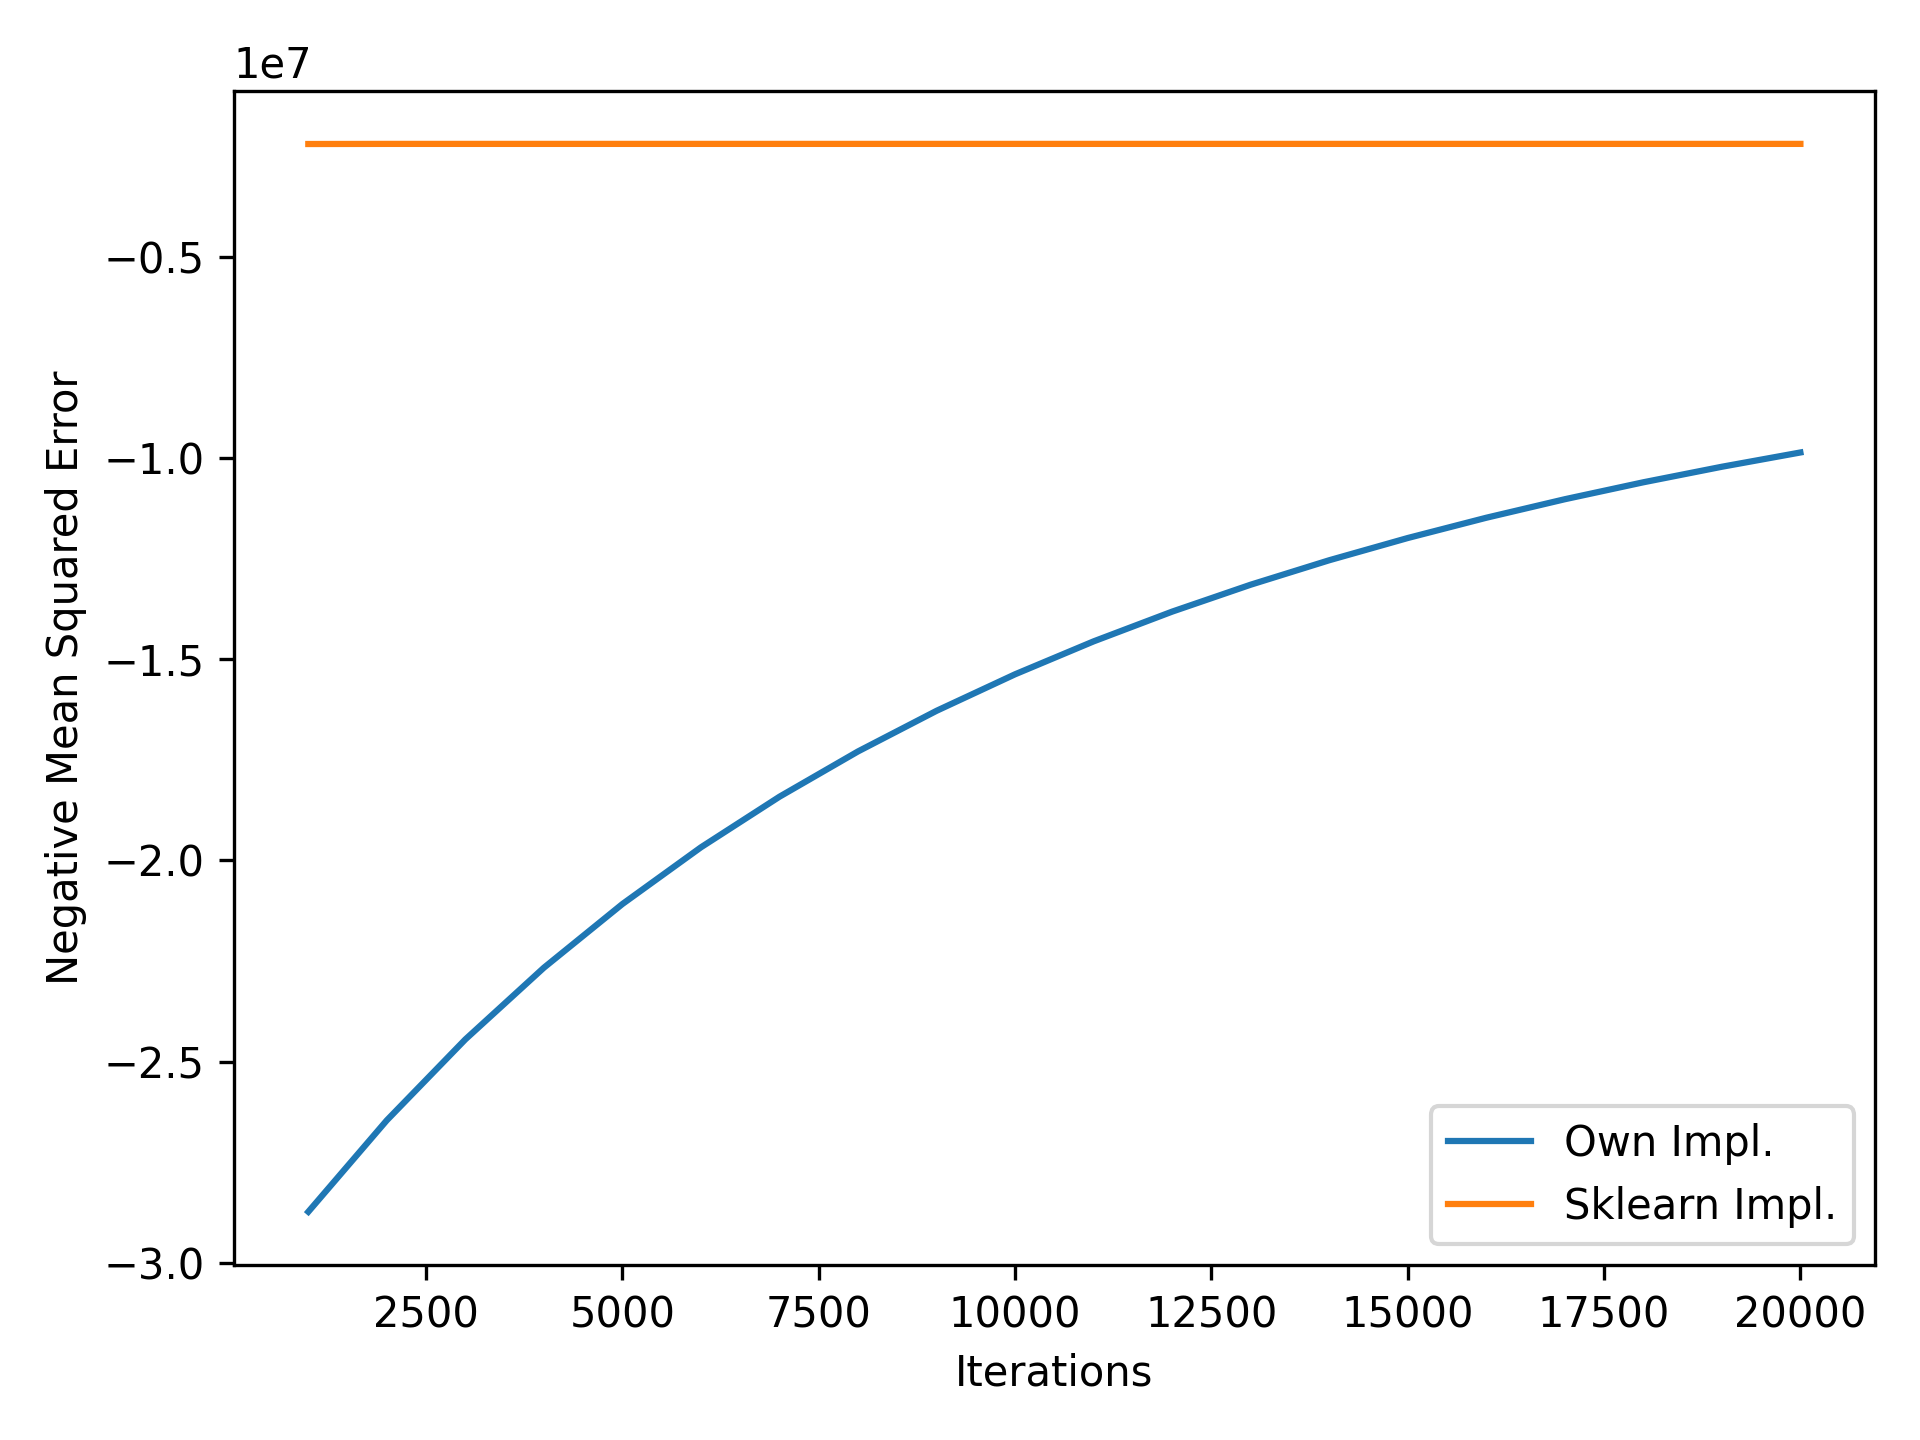
\includegraphics[width=0.8\textwidth]{exercise_2/presentation/figures/diamond_scores_mean_sq_err.png}
            \caption{Mean squared error of Gradient Descent on Diamonds Data Set}
            \label{fig:Grad_Diamond_MSE}
       \end{figure}
    \end{frame}
    
    \begin{frame}{Performance on Diamonds Data Set}
        \begin{figure}[h!]
            \centering
            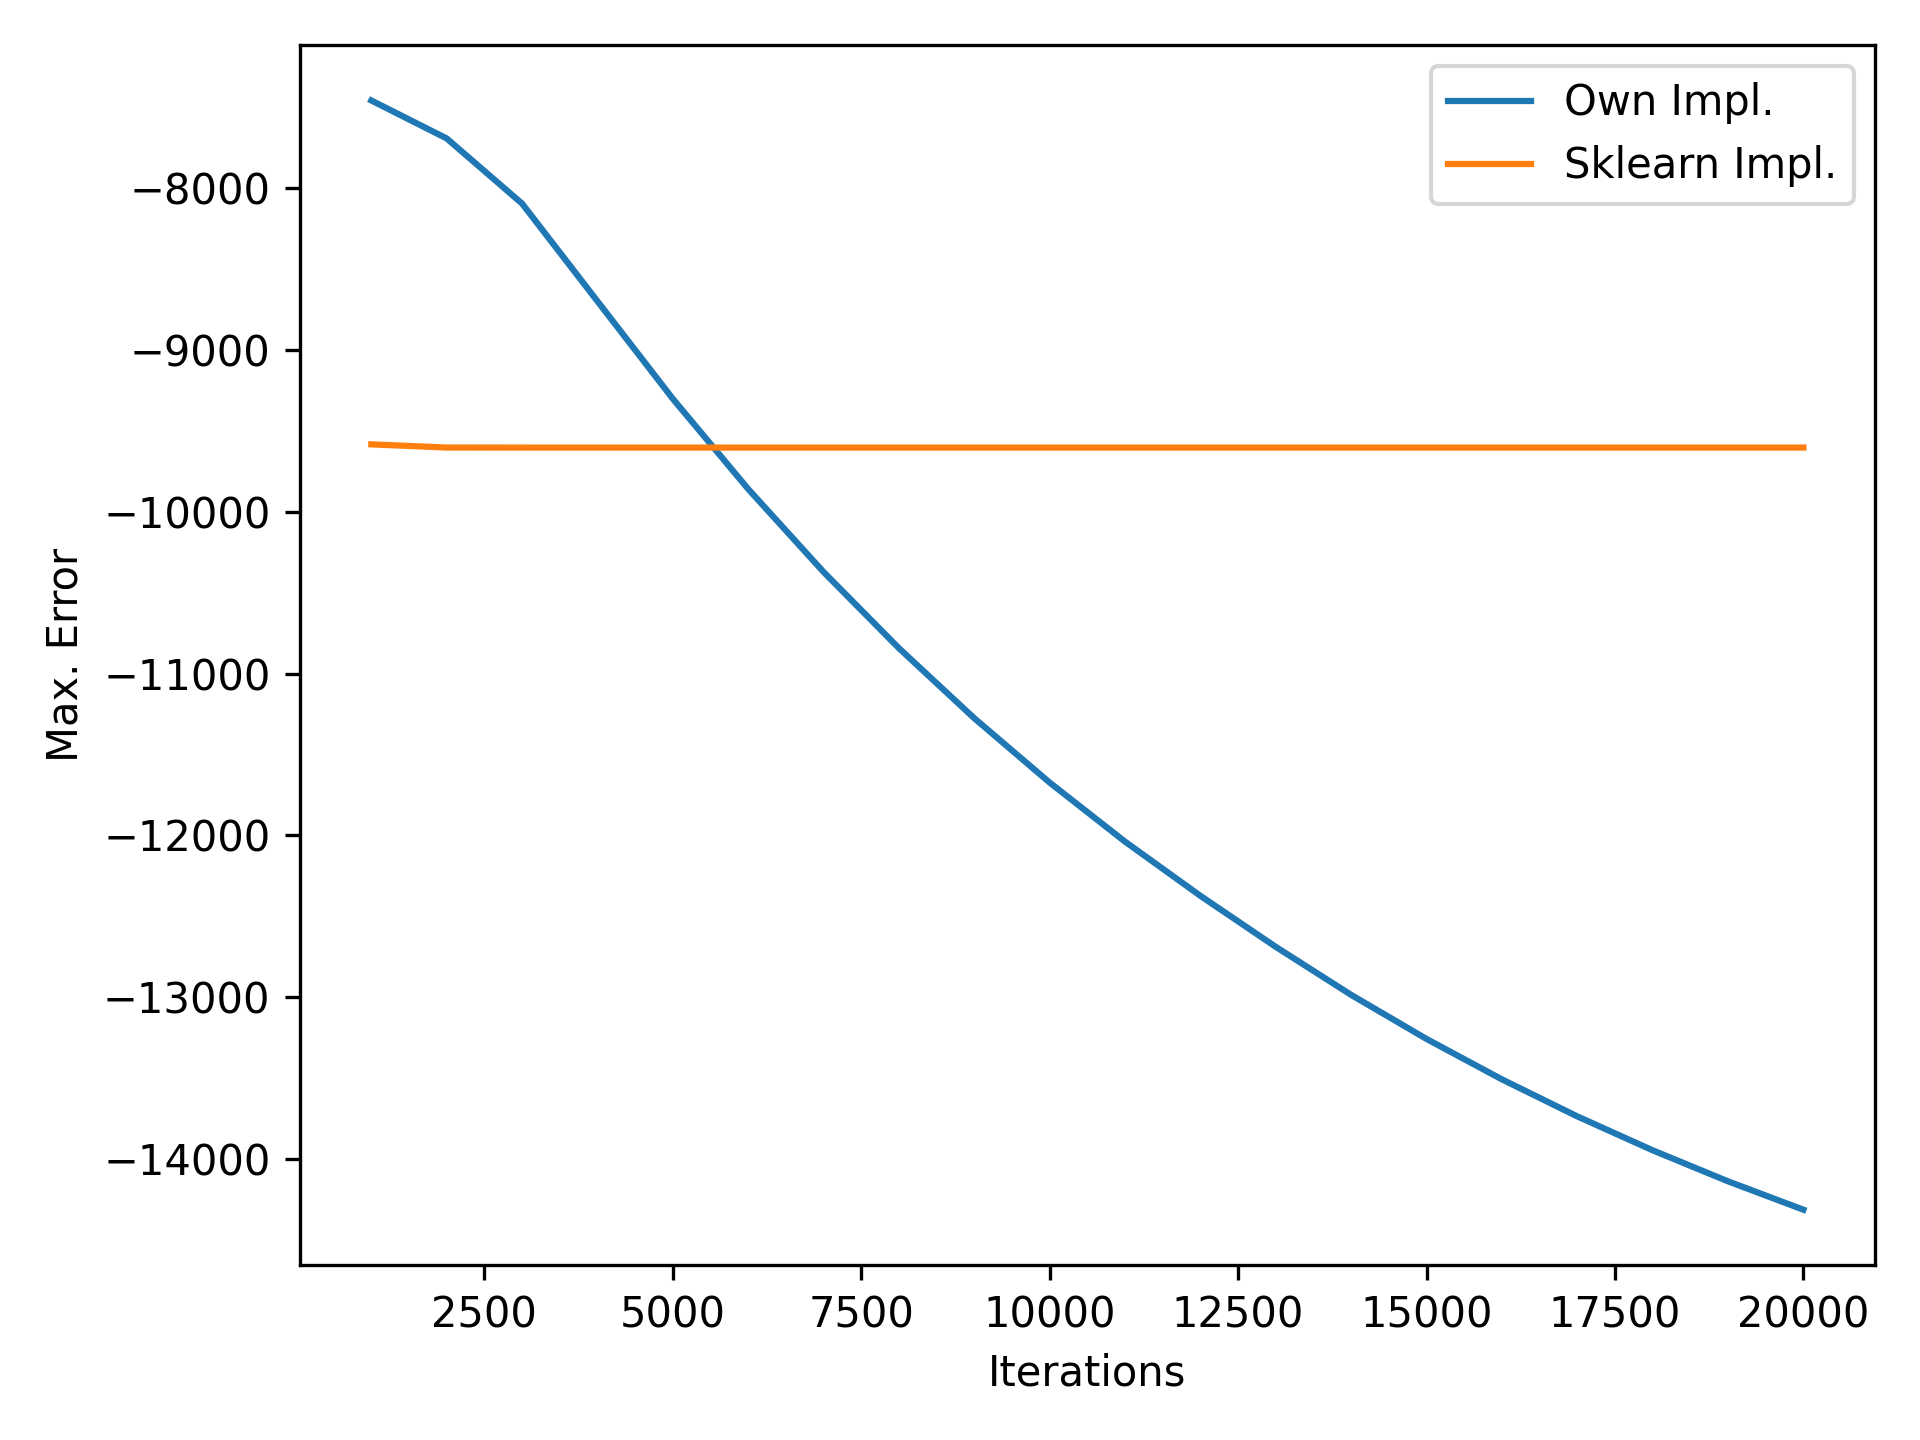
\includegraphics[width=0.8\textwidth]{exercise_2/presentation/figures/diamond_scores_max_error.png}
            \caption{Max. error of Gradient Descent on Diamonds Data Set}
            \label{fig:Grad_Diamond_max-error}
       \end{figure}
    \end{frame}
    
    \begin{frame}{Performance on Concrete Data Set}
        \begin{figure}[h!]
            \centering
            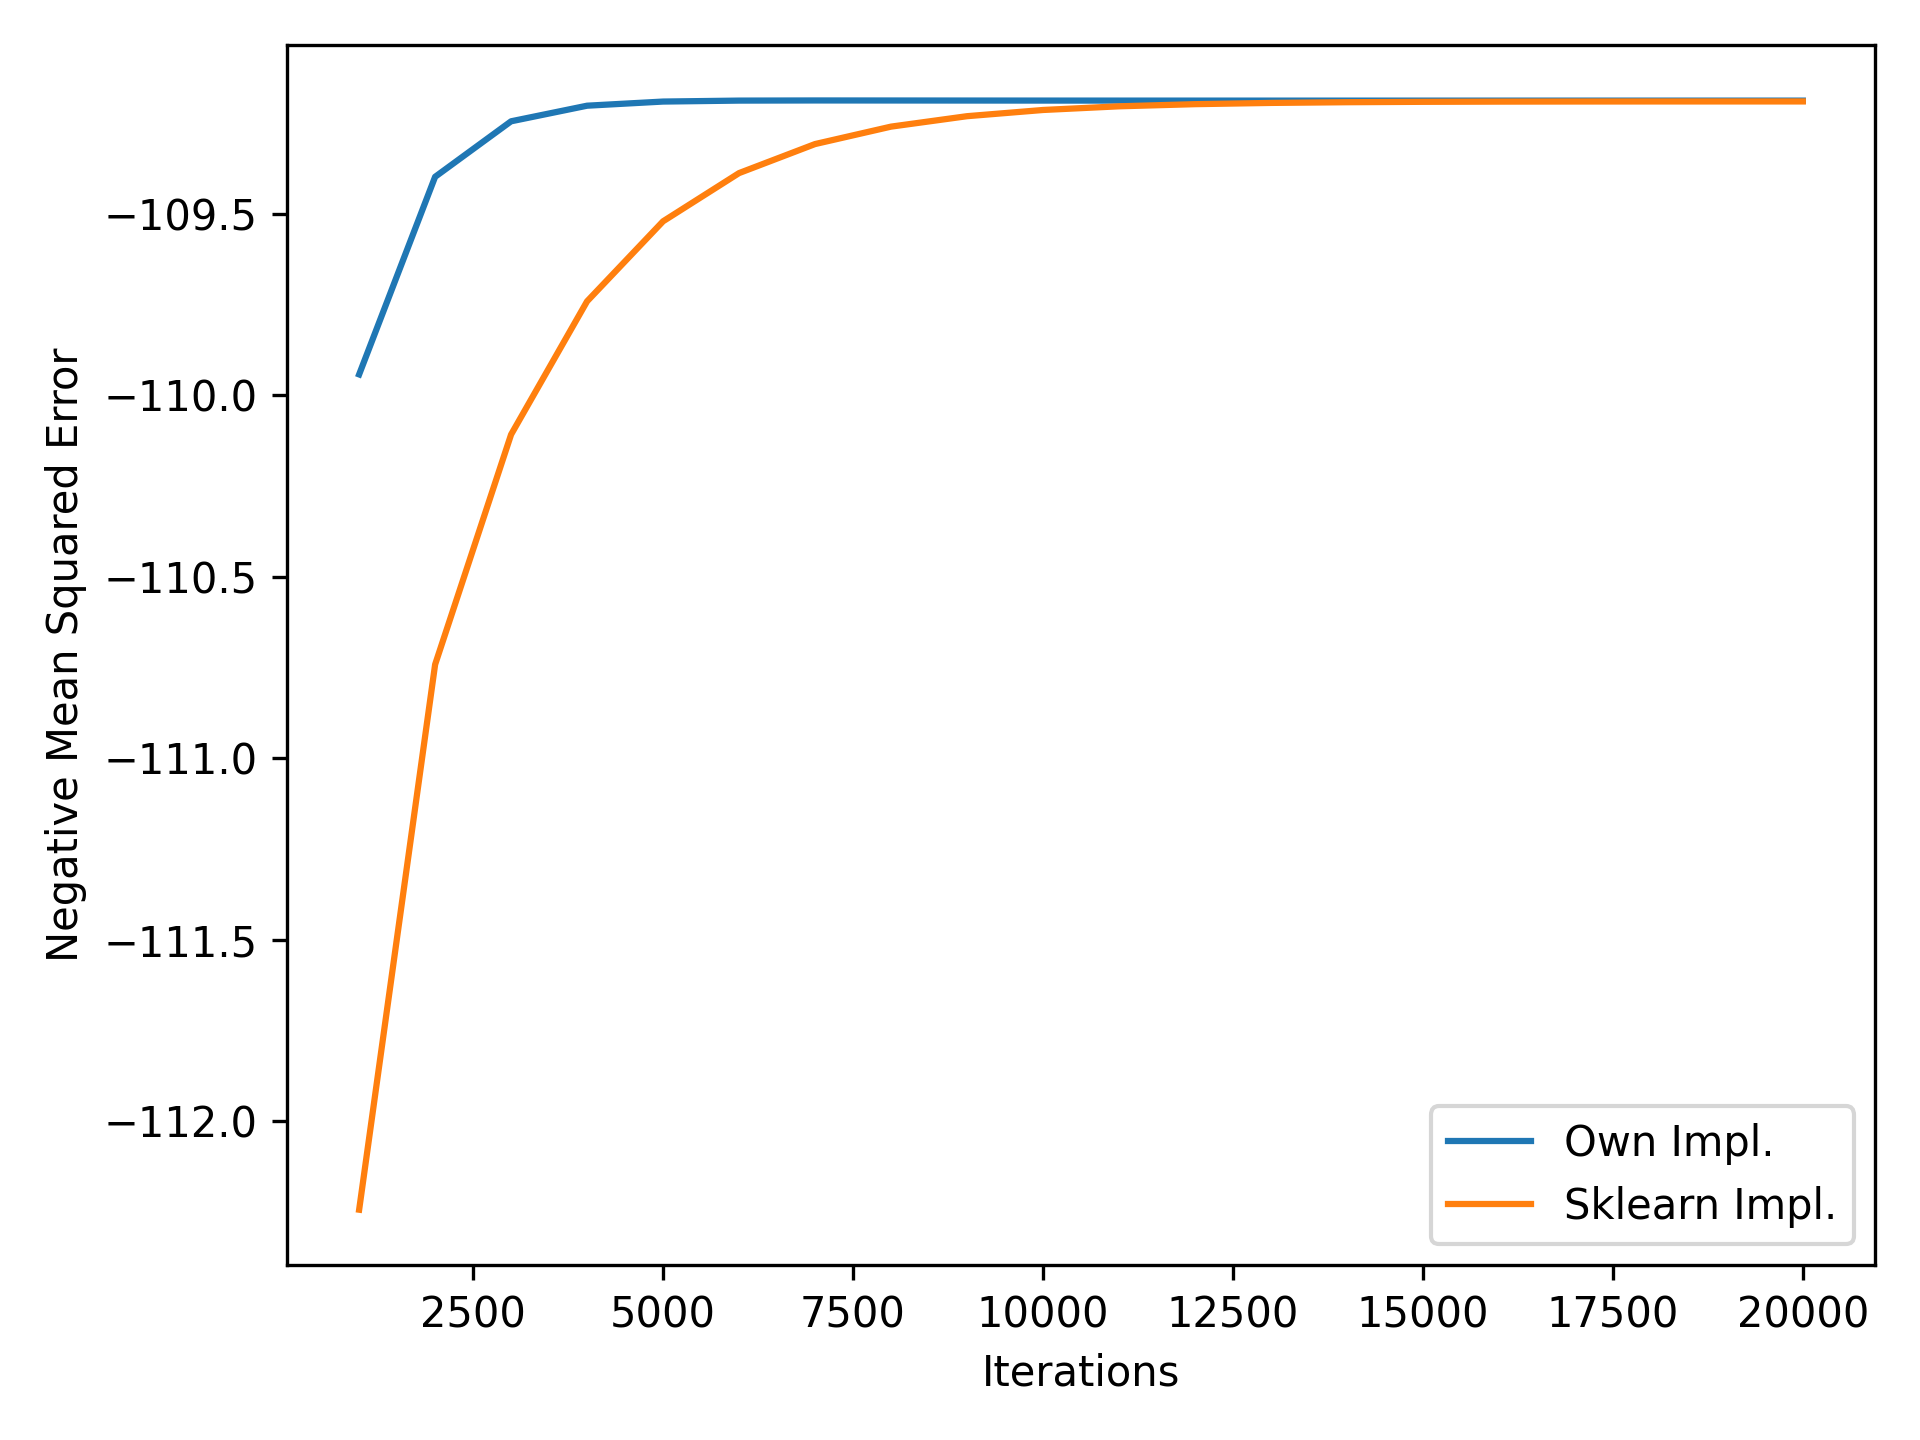
\includegraphics[width=0.8\textwidth]{exercise_2/presentation/figures/concrete_gradient-descent_scores_mean_sq_err.png}
            \caption{Mean squared error of Gradient Descent on Concrete Set}
            \label{fig:Grad_Concrete_MSE}
       \end{figure}    
    \end{frame}
    
    \begin{frame}{Performance on Concrete Data Set}
        \begin{figure}[h!]
            \centering
            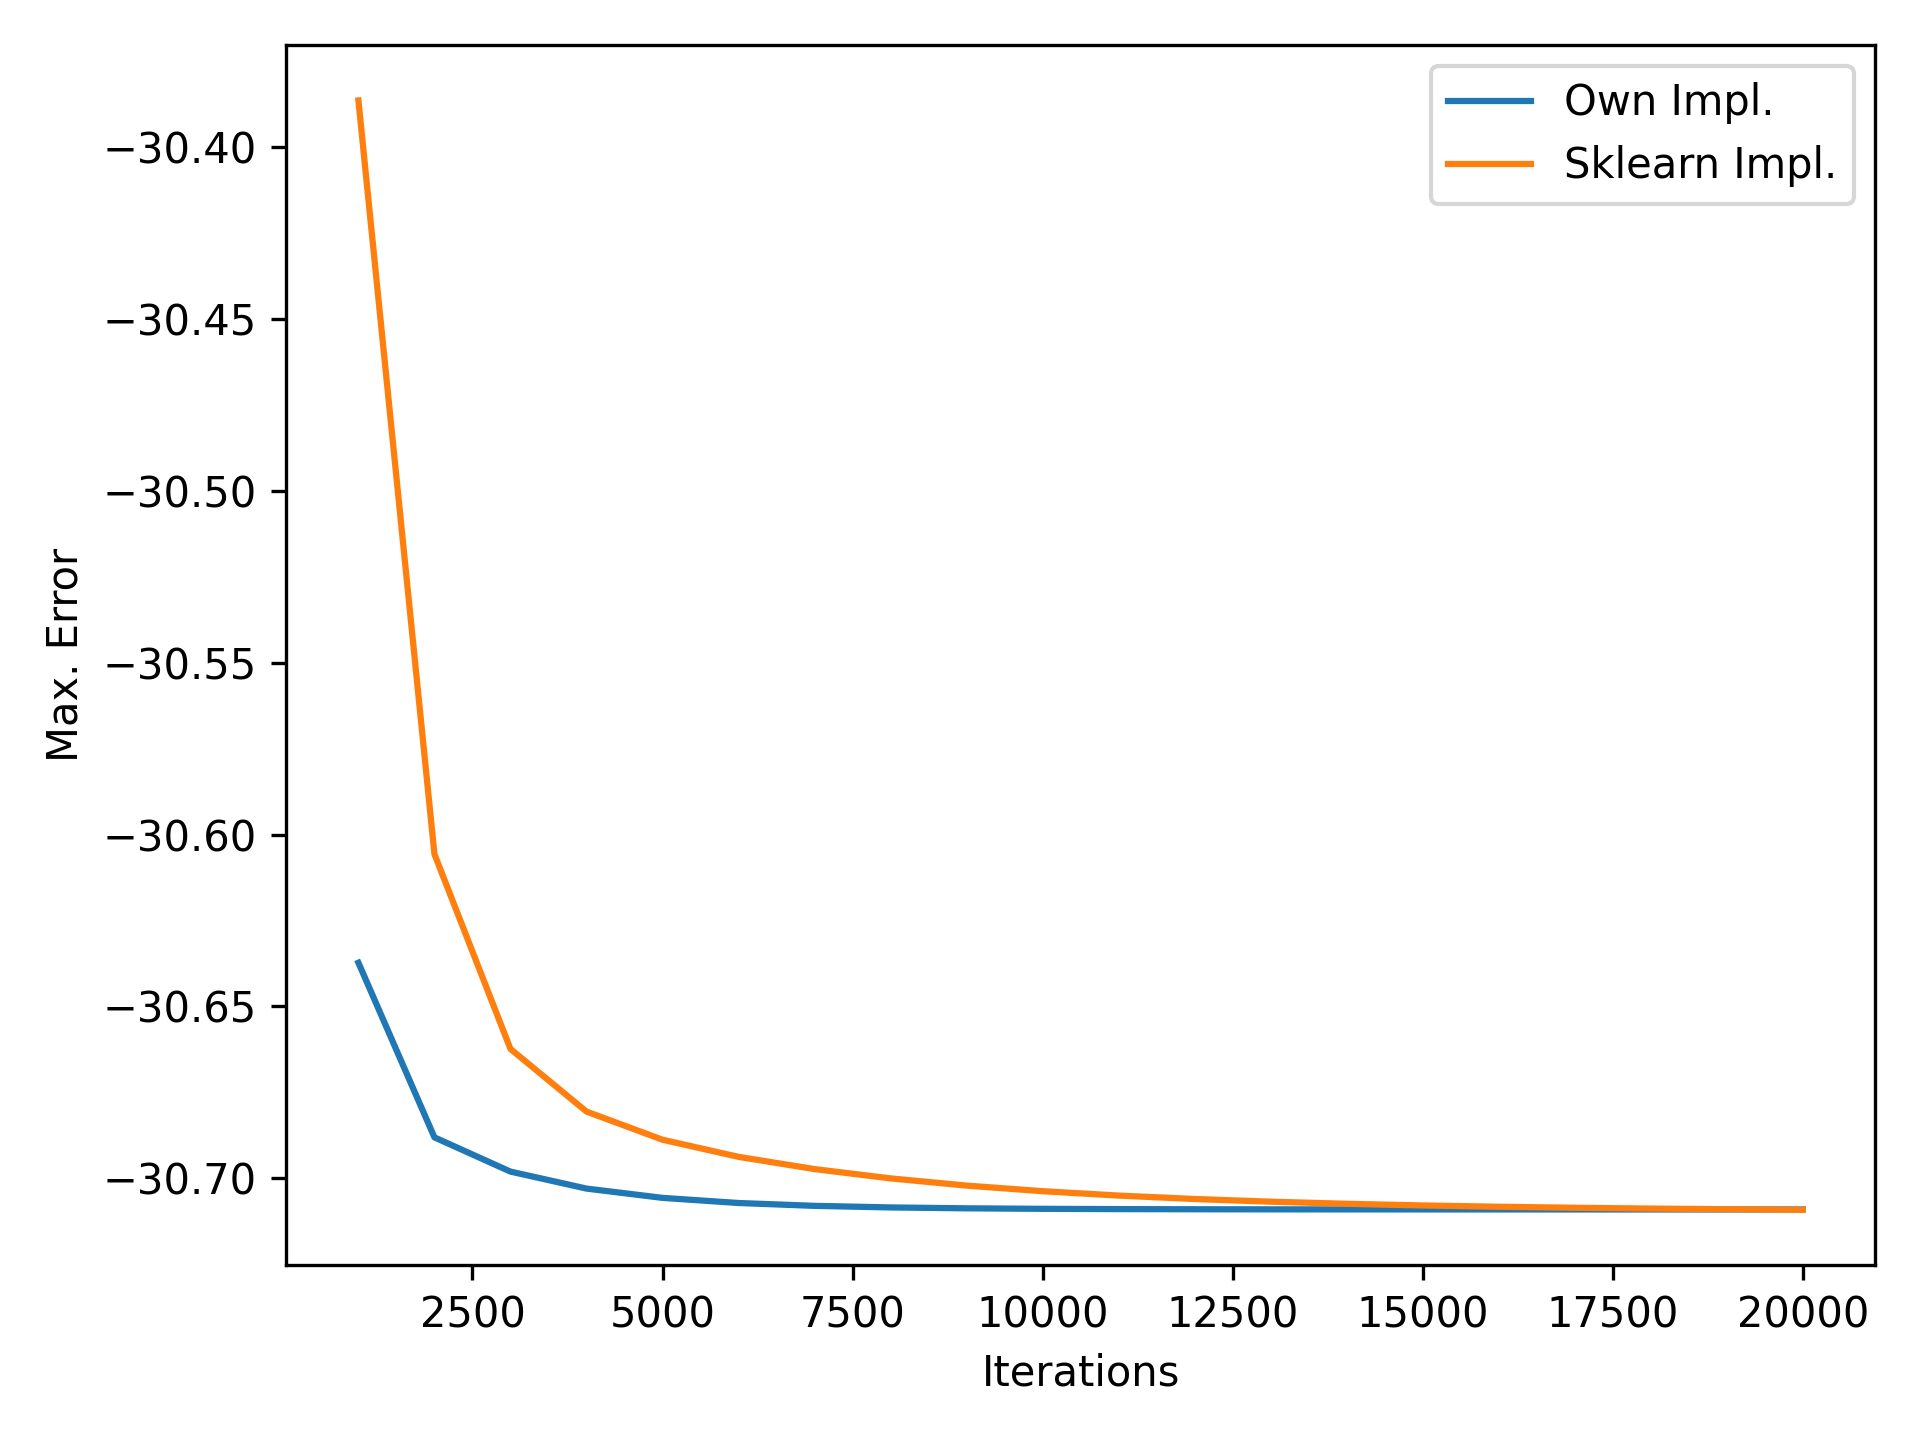
\includegraphics[width=0.8\textwidth]{exercise_2/presentation/figures/concrete_gradient-descent_scores_max_error.png}
            \caption{Max. error of Gradient Descent on Concrete Set}
            \label{fig:Grad_Concrete_max-error}
        \end{figure}        
    \end{frame}
    
    \begin{frame}{Performance on Life Expectancy Data Set}
        \begin{figure}[h!]
            \centering
            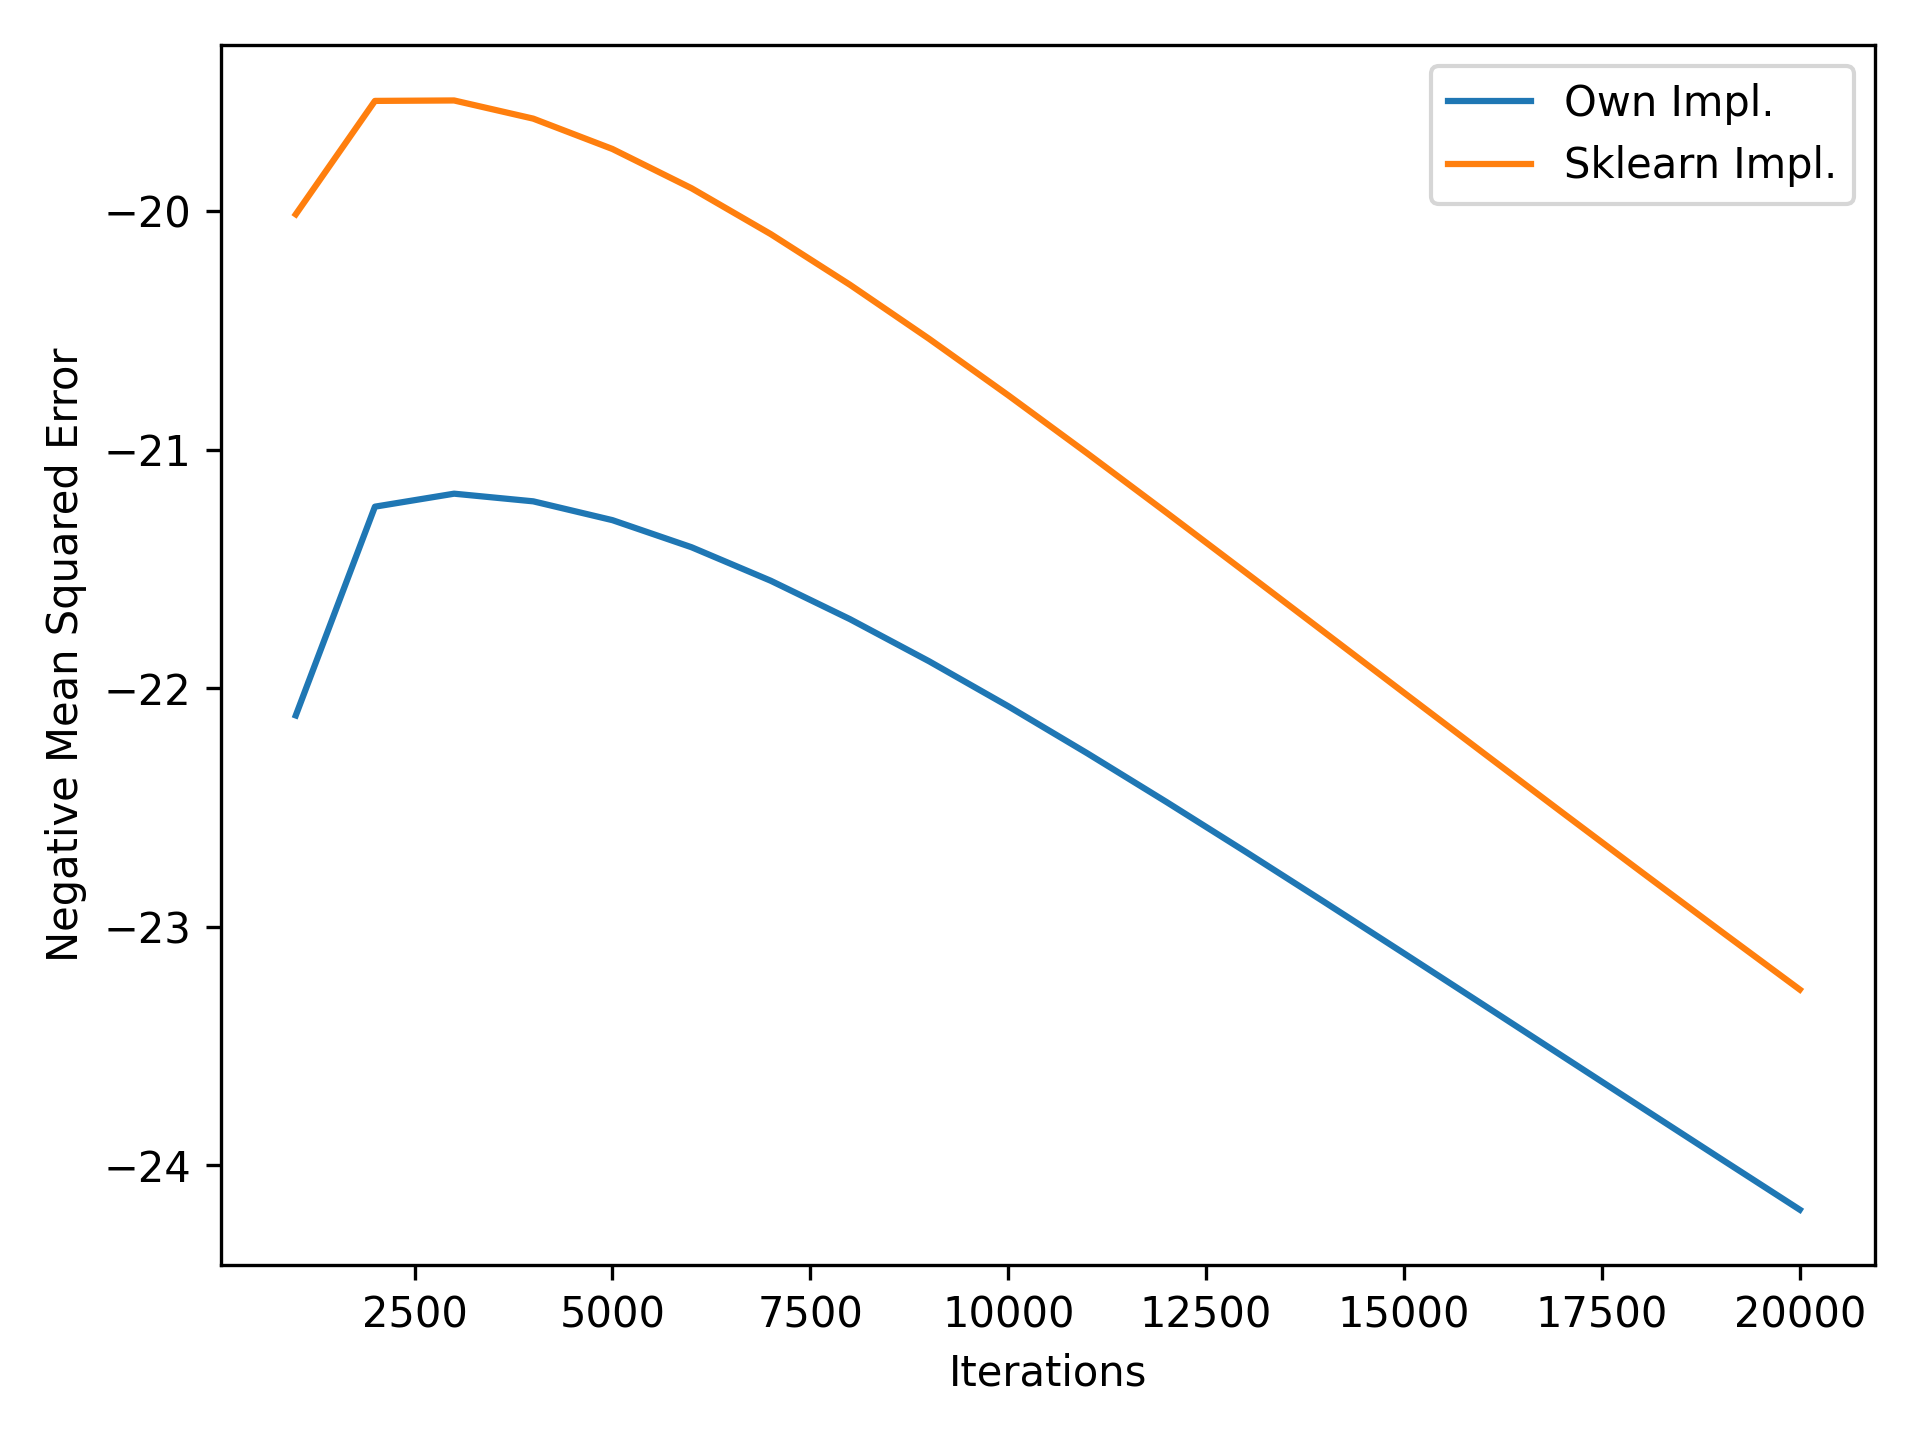
\includegraphics[width=0.8\textwidth]{exercise_2/presentation/figures/le_gradient-descent_scores_mean_sq_err.png}
            \caption{MSE of Gradient Descent on Life Expectancy Data Set}
            \label{fig:Grad_LE_MSE}
       \end{figure}    
    \end{frame}
    
    \begin{frame}{Performance on Life Expectancy Data Set}
          \begin{figure}[h!]
            \centering
            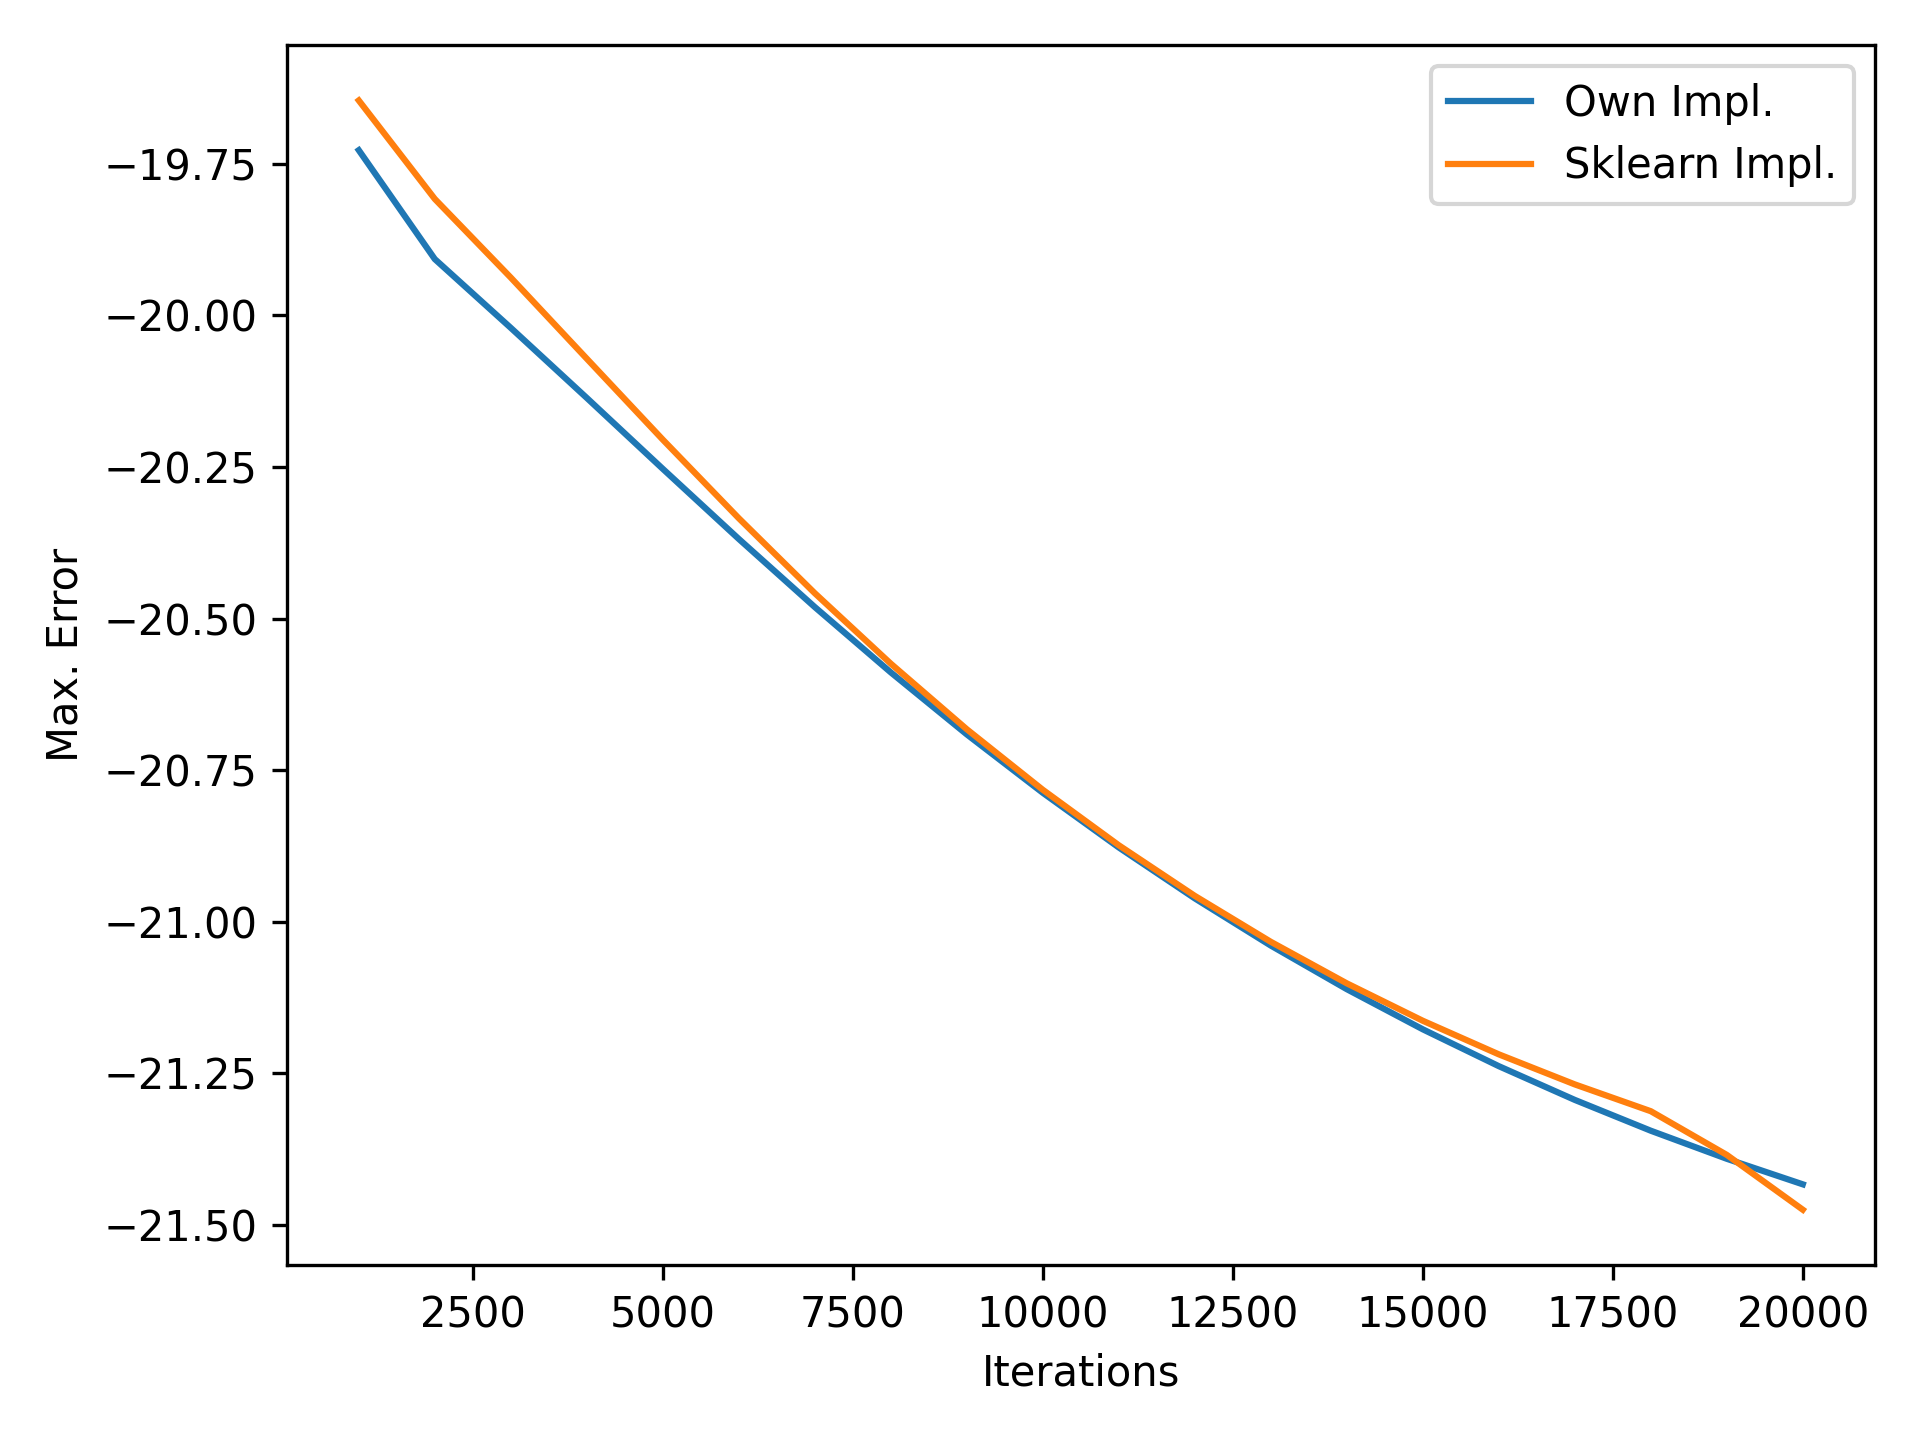
\includegraphics[width=0.8\textwidth]{exercise_2/presentation/figures/le_gradient-descent_scores_max_error.png}
            \caption{Max. error of Gradient Descent on Life Expectancy Data Set}
            \label{fig:Grad_LE_max-error}
       \end{figure}
    \end{frame}
    
    \begin{frame}{Runtime on Diamonds Data Set}
        \begin{figure}[h!]
            \centering
            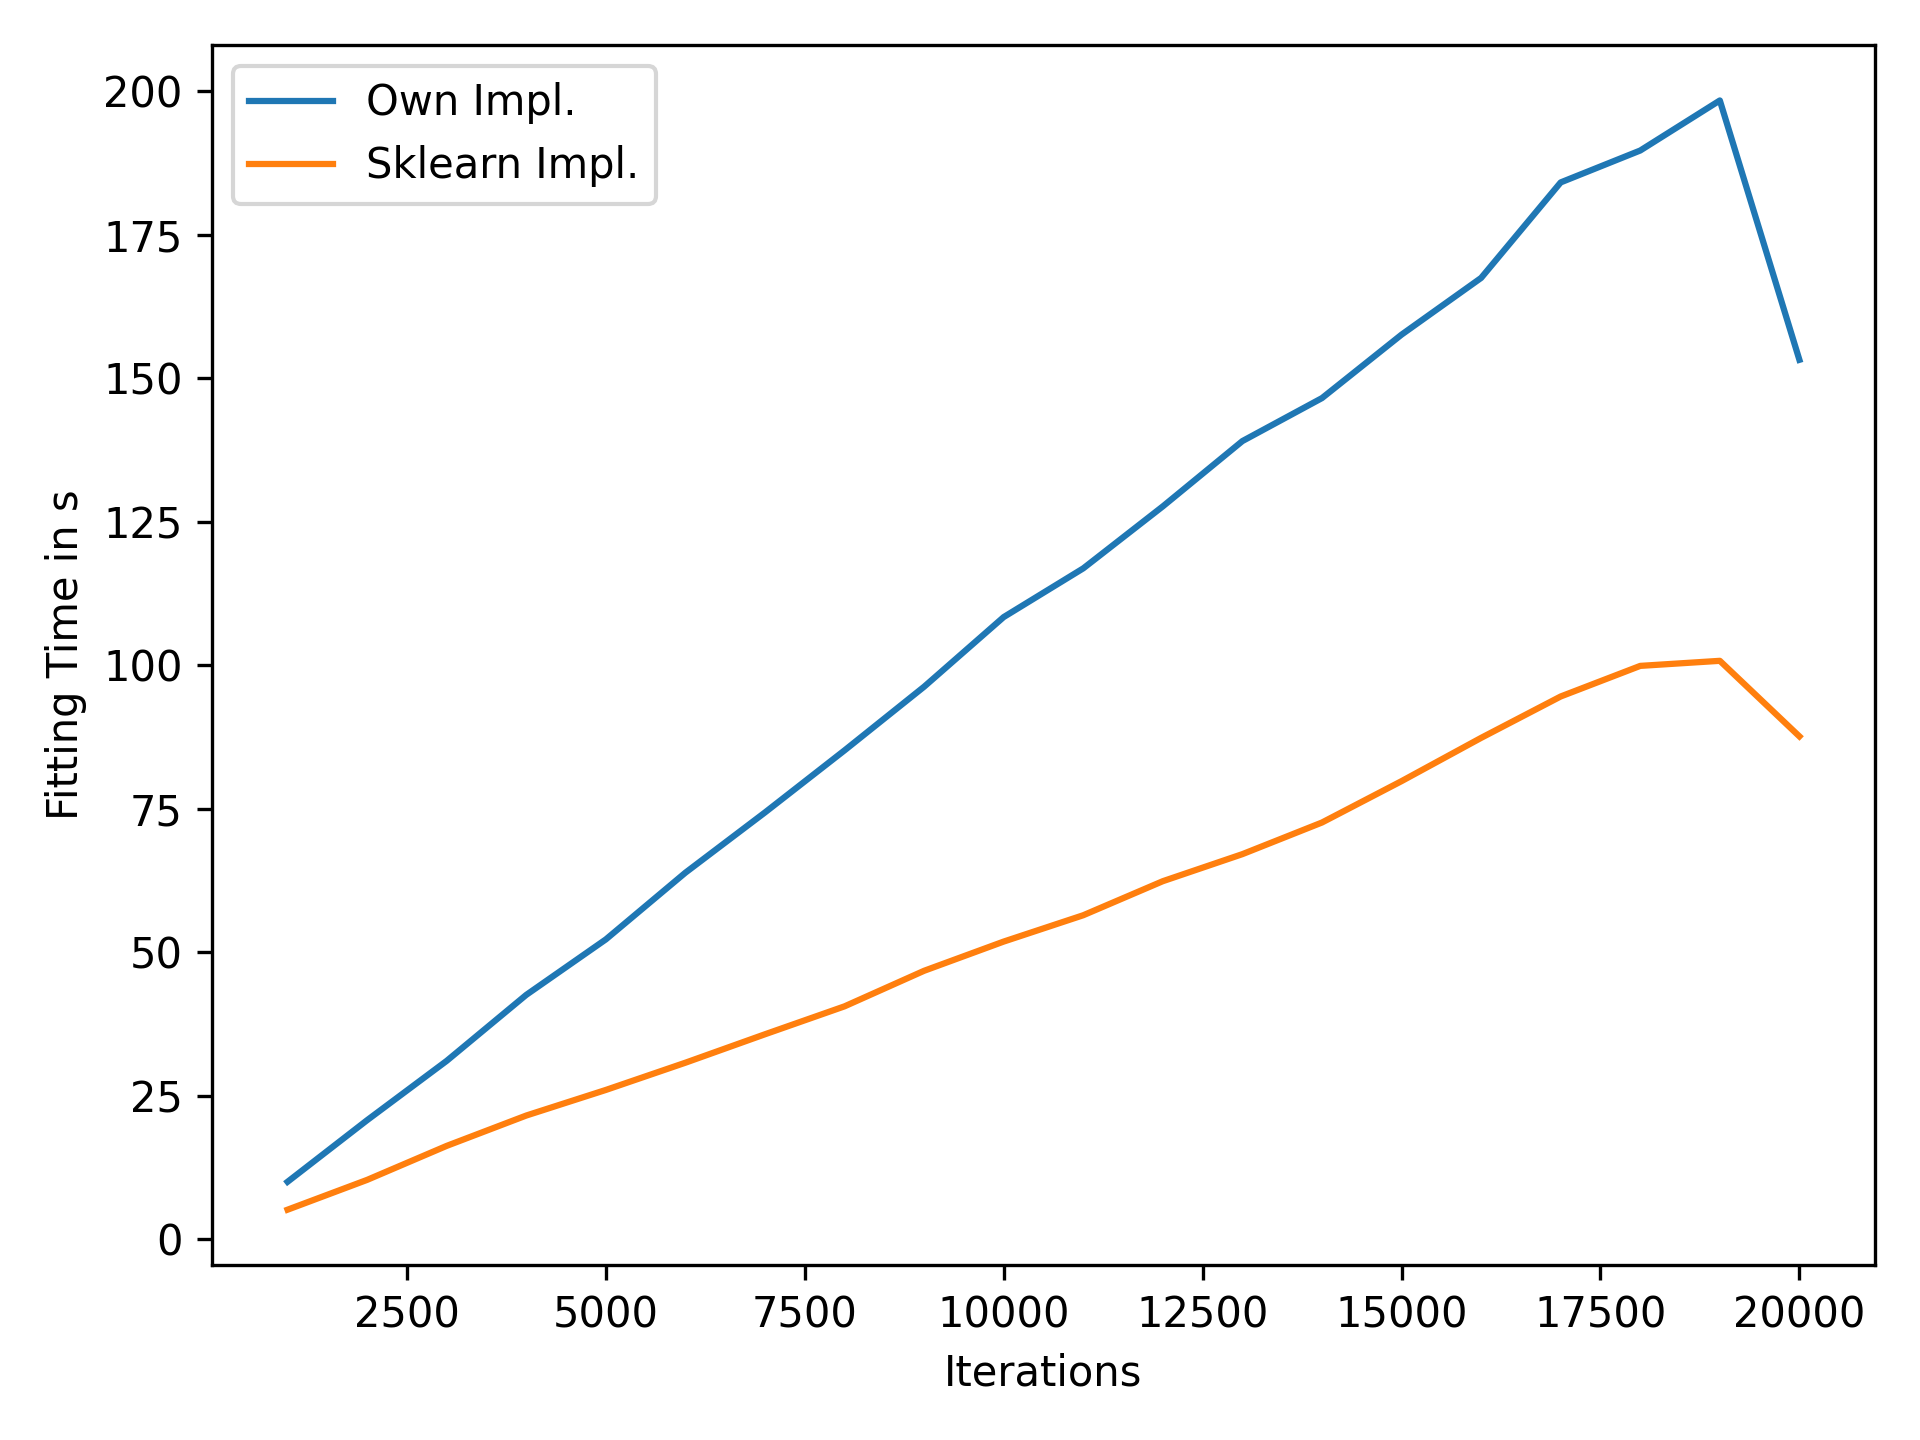
\includegraphics[width=0.8\textwidth]{exercise_2/presentation/figures/diamond_scores_runtime.png}
            \caption{Runtime of Gradient Descent on Diamonds Data Set}
            \label{fig:Grad_Diamond_runtime}
       \end{figure}
    \end{frame}
    
    \begin{frame}{Runtime on Concrete Data Set}
        \begin{figure}[h!]
            \centering
            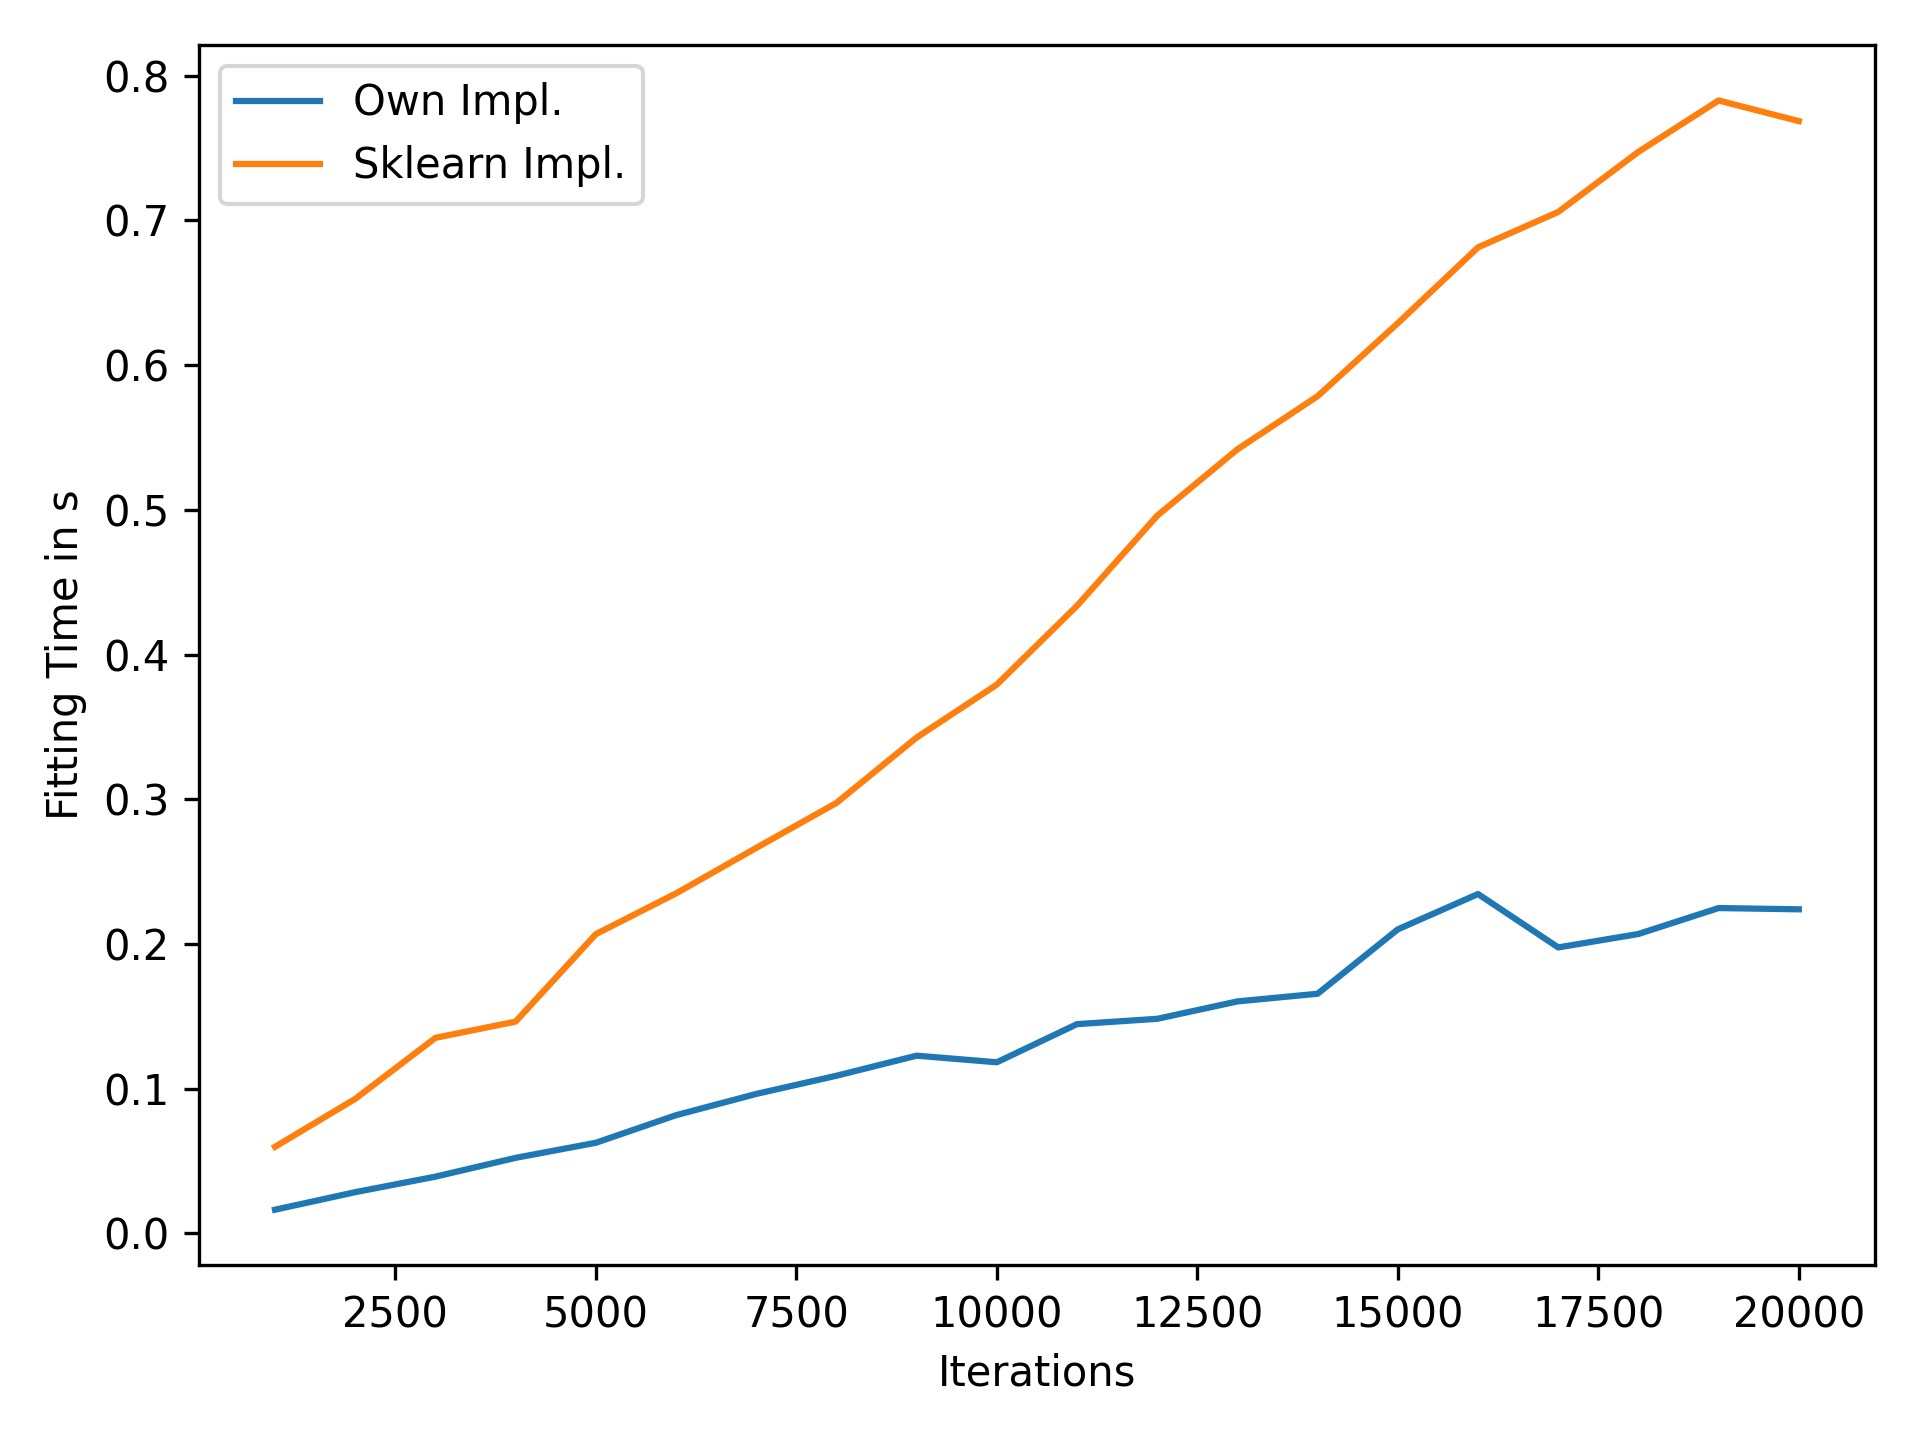
\includegraphics[width=0.8\textwidth]{exercise_2/presentation/figures/concrete_gradient-descent_scores_runtime.png}
            \caption{Runtime of Gradient Descent on Concrete Data Set}
            \label{fig:Grad_Concrete_runtime}
       \end{figure}        
    \end{frame}
    
    \begin{frame}{Runtime on Life Expectancy Data Set}
          \begin{figure}[h!]
            \centering
            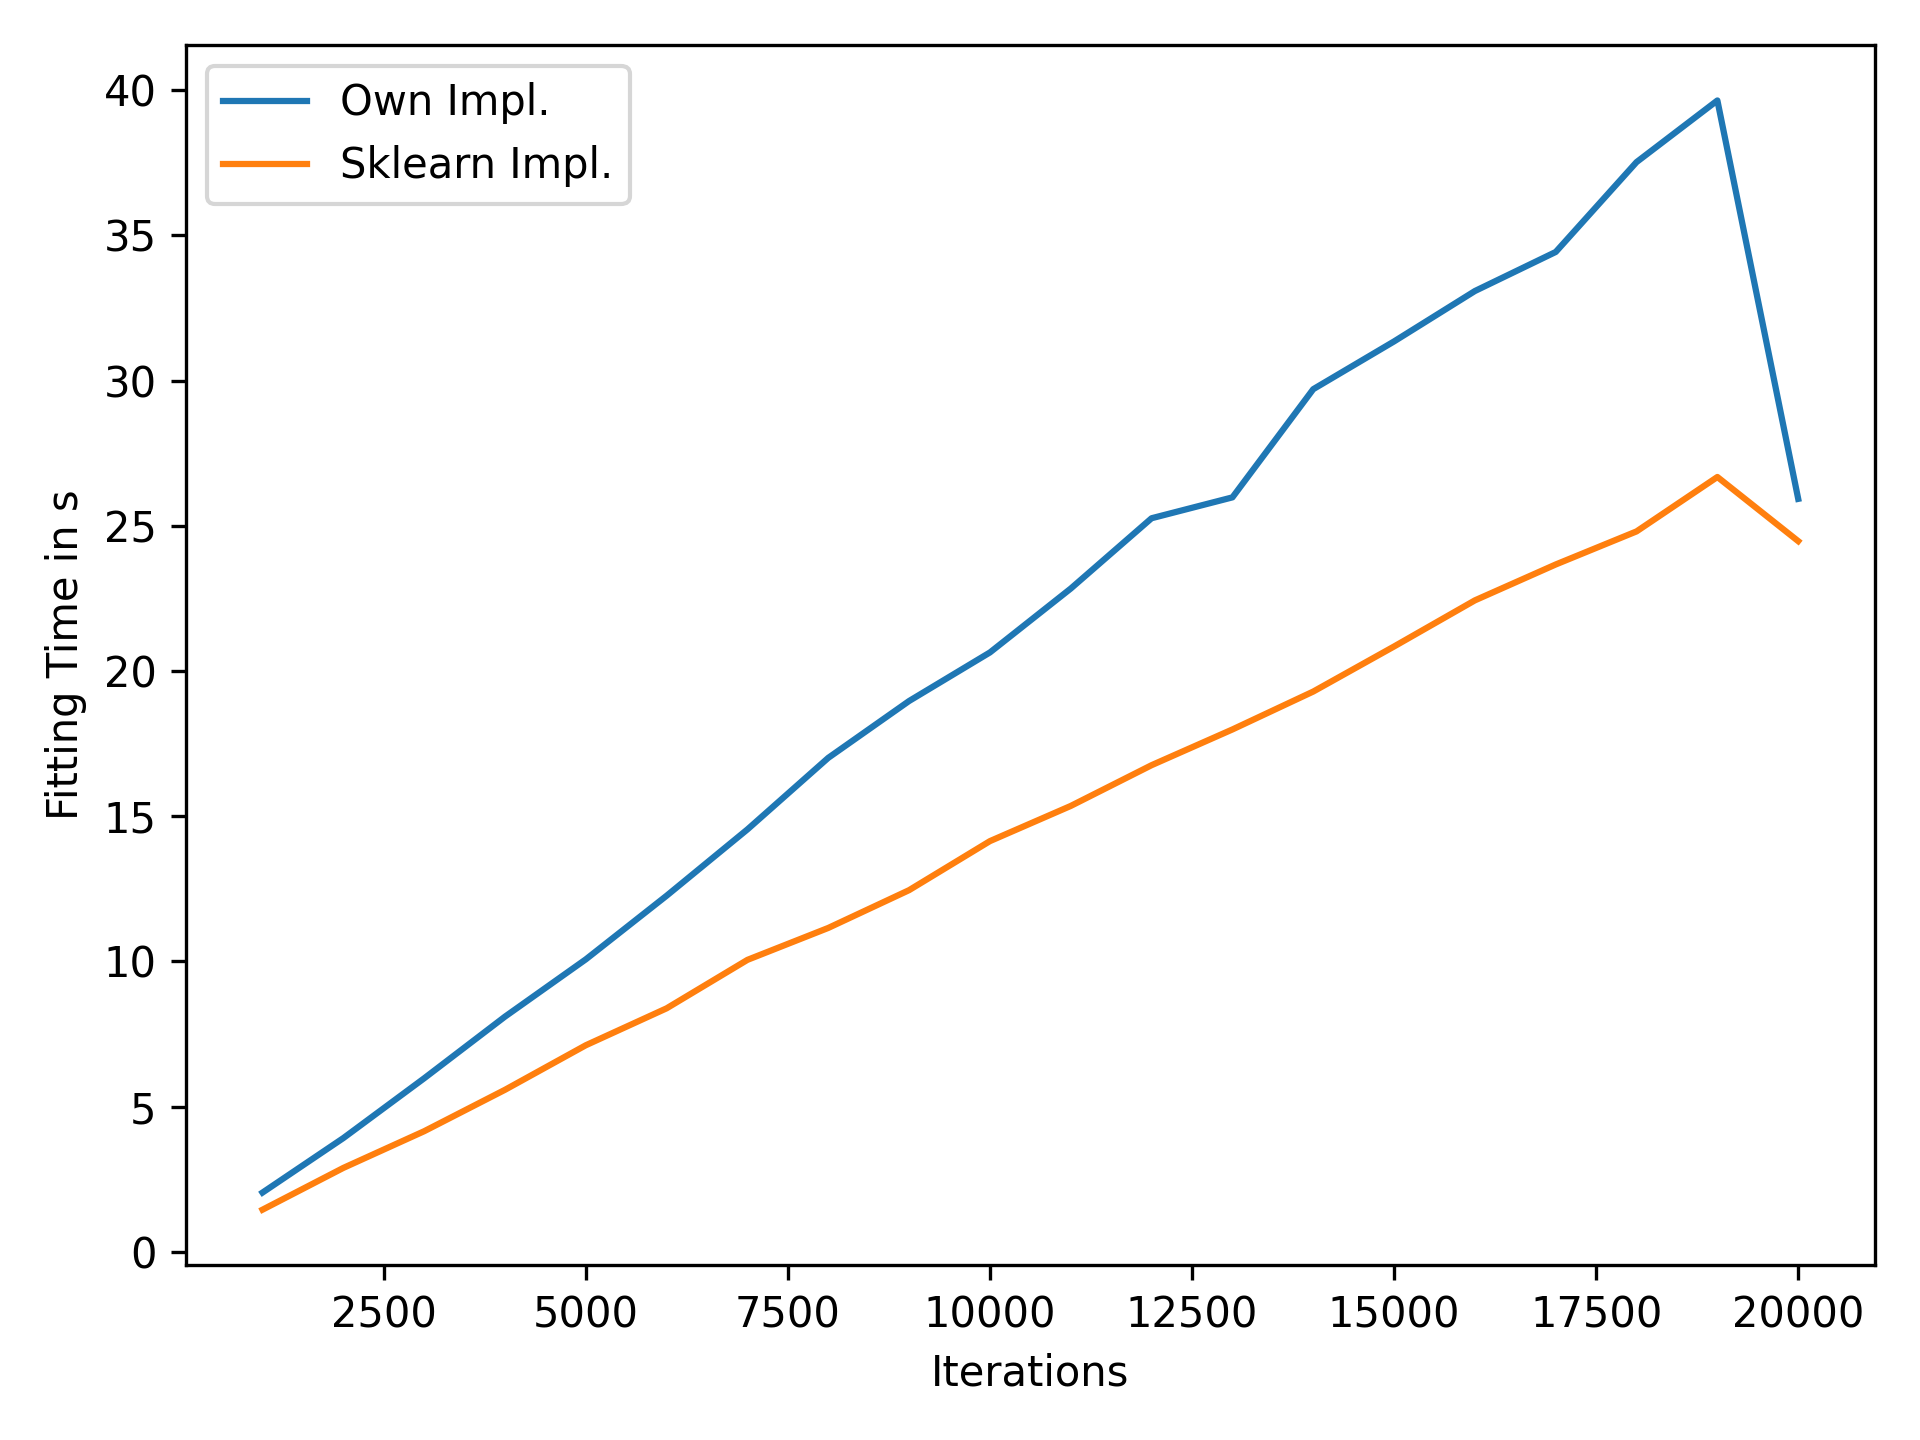
\includegraphics[width=0.8\textwidth]{exercise_2/presentation/figures/le_gradient-descent_scores_runtime.png}
            \caption{Runtime of Gradient Descent on Life expectancy Data Set}
            \label{fig:Grad_LE_runtime}
       \end{figure}
    \end{frame}
    
\section[$k$-NN]{$k$-NN Algorithm}
    \begin{frame}[fragile]{$k$-NN}
        $n$ = \#attributes
        
        Distance functions (using numpy.linalg.norm in Python):
            \begin{enumerate}
                \item Manhattan distance: $d_1(x_1, x_2) = \sum_{i=1}^n |x_{1i} - x_{2i}|$
                \item Euclidean distance: $d_2(x_1, x_2) = \sqrt{\sum_{i=1}^n (x_{1i} - x_{2i})^2}$
                \item Chebyshev distance: $d_\infty(x_1, x_2) = \max_{i \in \{1,...,n\}}|x_{1i} - x_{2i}|$
            \end{enumerate}
        
        Weight:
            \begin{enumerate}
                \item Uniform $\rightarrow$ mean of predicted class of $k$ nearest neighbours
                \item Distance based: $\frac{1}{d(x_1, x_2)+\varepsilon}$ (very small $\varepsilon>0$ to prevent division by $0$) $\rightarrow$ weighted mean of predicted class of $k$ nearest neighbours
            \end{enumerate}
    \end{frame}
    
    \begin{frame}[fragile]{$k$-NN: Pseudocode}
        \begin{algorithm}[H]
            \caption{$k$-NN-Regressor($k$, distance-fct $d$, weight, $X_{t}$, $Y_{t}$, $x_{p}$)}
			\begin{algorithmic}[1]
			    \State neighbors = [\,]
			    \Comment Initialize min-heap
			    \For{each row ($x$,$y$) in ($X_{t}$, $Y_{t}$)}
			    \Comment Find $k$ nearest neighbors
			        \State distance\textunderscore tuple = ($-d(x, x_{p}), x, y$)
			        \If{$|\text{neighbors}|<k$}
			            \State push(neighbors, distance\textunderscore tuple)
			        \Else
			            \State pushpop(neighbors, distance\textunderscore tuple)
			        \EndIf
			    \EndFor
			    \If{weight='uniform'}
			    \Comment Prediction
			        \State prediction $= \frac{1}{k}\sum_{i=1}^k$ neighbors$[i][2]$
			    \ElsIf{weight='distance'}
			        \State prediction $= \frac{\sum_{i=1}^k neighbors[i][0] \cdot neighbors[i][2]}{\sum_{i=1}^k neighbors[i][0]}$
			    \EndIf
			    \State \Return prediction
			\end{algorithmic}
		\end{algorithm}
    \end{frame}
    
    \begin{frame}[fragile]{Results}
        \begin{itemize}
            \item Distance function:
                \begin{enumerate}
                    \item For Diamonds and Life Expectancy data set: Manhattan distance best results, but Euclidean distance also pretty good
                    \item For Concrete data set: Euclidean distance best, but Manhattan also good
                    \item Chebyshev distance generally not optimal for our data sets
                \end{enumerate}
            \item $k$ value:
                \begin{enumerate}
                    \item Not the same optimal $k$ value for all our data sets
                \end{enumerate}
            
            \item Scaling:
                \begin{enumerate}
                    \item Best results for all data sets obtained with standard-Scaling
                    \item Min-Max-Scaler resp. without scaling not really good
                \end{enumerate}
        \end{itemize}
    \end{frame}
    
    \begin{frame}{Performance on Diamonds Data Set}
        \begin{figure}[h!]
            \centering
            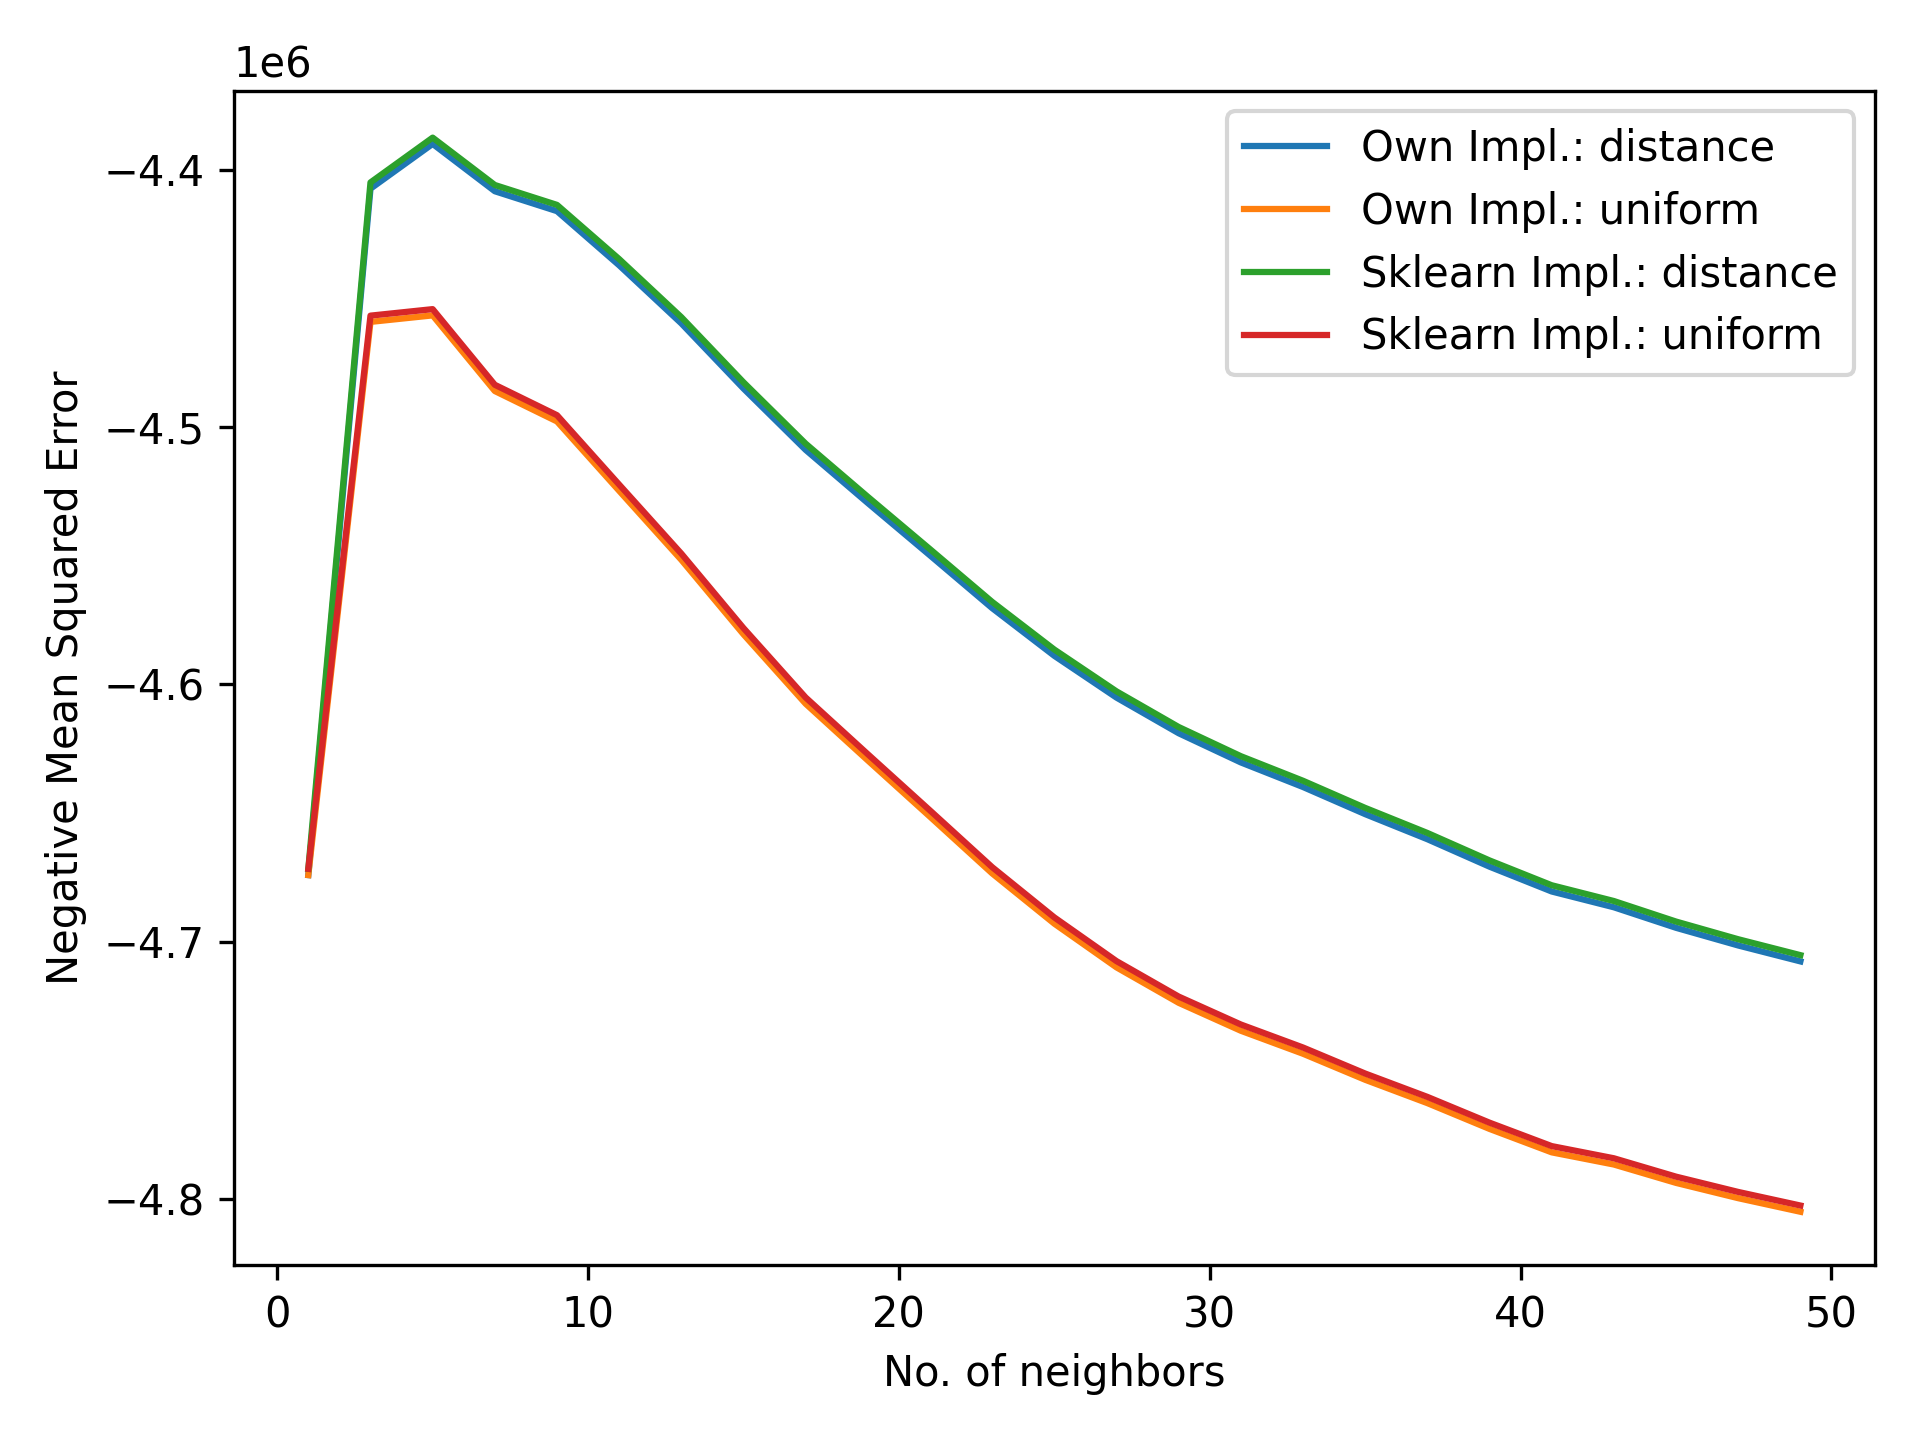
\includegraphics[width=0.8\textwidth]{exercise_2/presentation/figures/diamond_knn_scores_mean_sq_err.png}
            \caption{Mean squared error of $k$-NN on Diamonds Data Set}
            \label{fig:kNN_Diamond_MSE}
       \end{figure}
    \end{frame}
    
    \begin{frame}{Performance on Diamonds Data Set}
        \begin{figure}[h!]
            \centering
            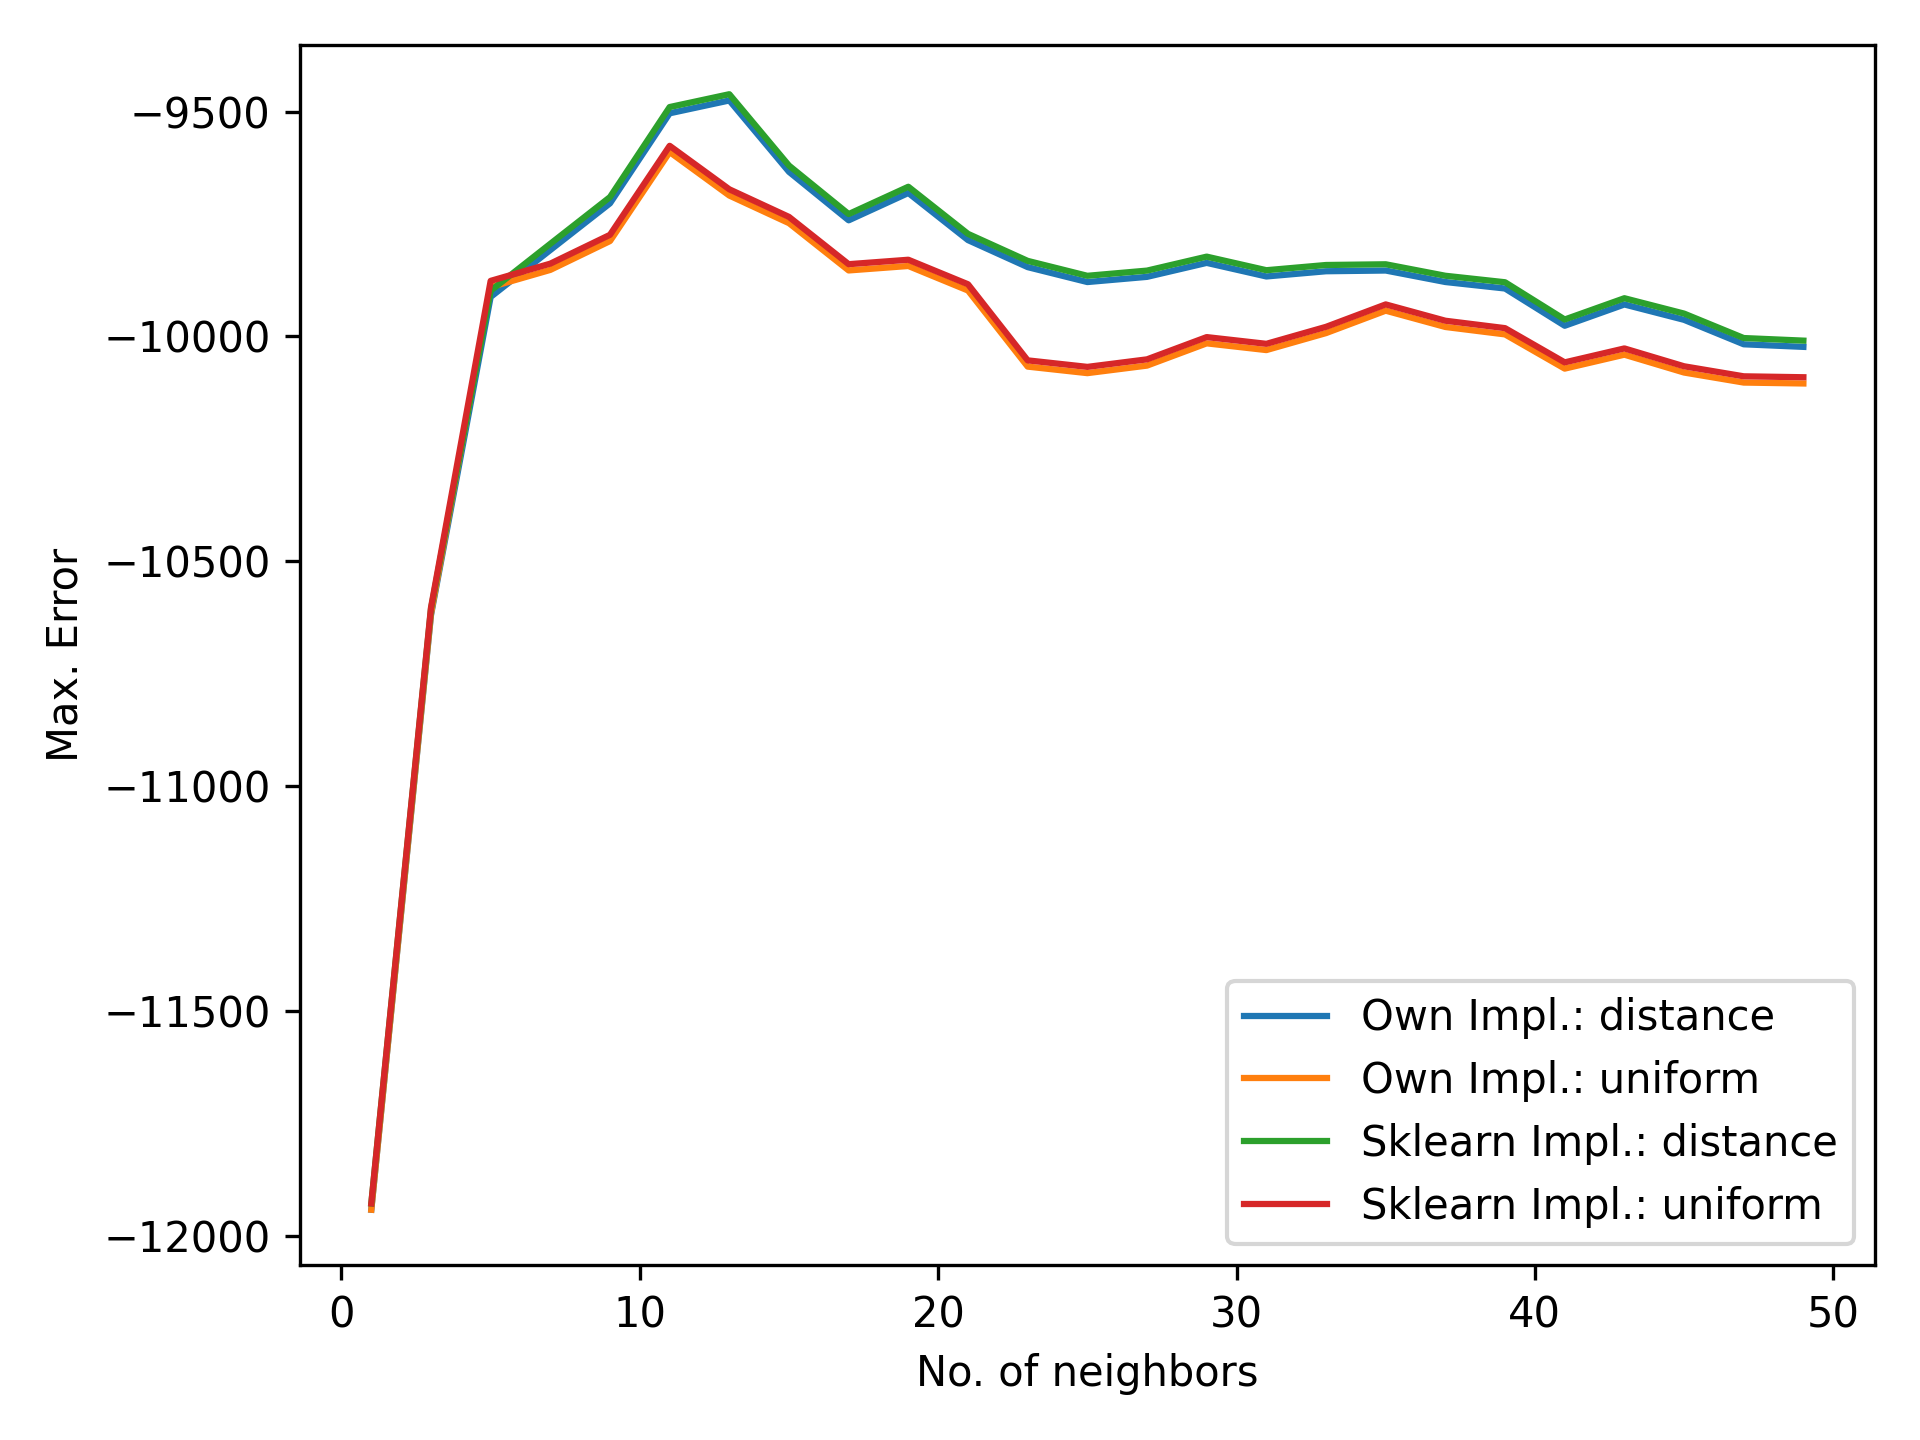
\includegraphics[width=0.8\textwidth]{exercise_2/presentation/figures/diamond_knn_scores_max_error.png}
            \caption{Max. error of $k$-NN on Diamonds Data Set}
            \label{fig:kNN_Diamond_max-error}
       \end{figure}
    \end{frame}
    
    
    \begin{frame}{Performance on Concrete Data Set}
        \begin{figure}[h!]
            \centering
            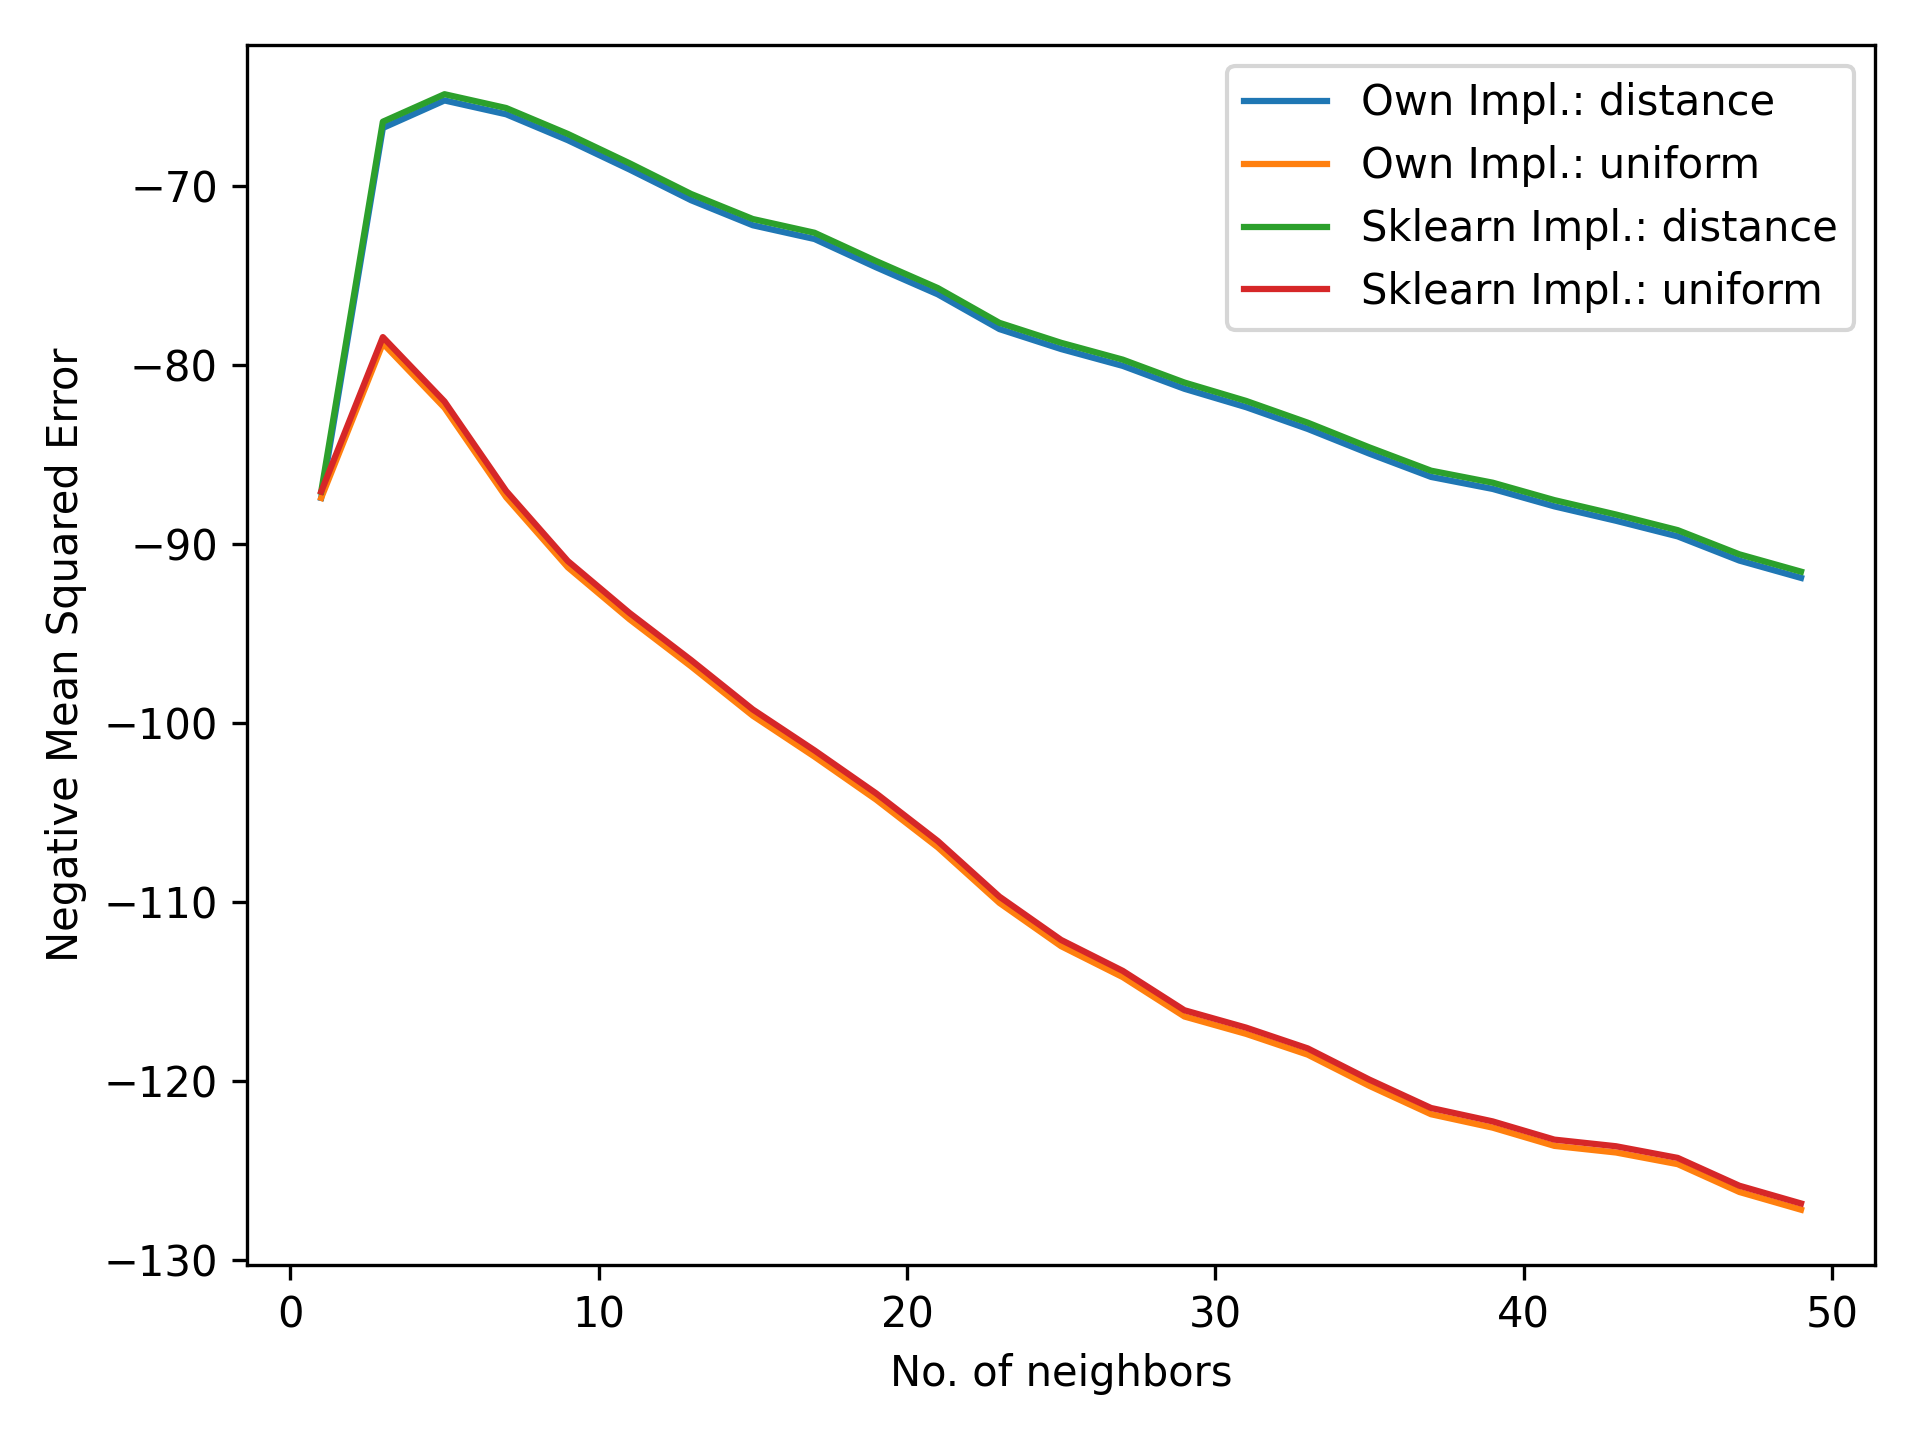
\includegraphics[width=0.8\textwidth]{exercise_2/presentation/figures/concrete_knn_scores_mean_sq_err.png}
            \caption{Mean squared error of $k$-NN on Concrete Data Set}
            \label{fig:kNN_concrete_MSE}
       \end{figure}
    \end{frame}
    
    \begin{frame}{Performance on Concrete Data Set}
        \begin{figure}[h!]
            \centering
            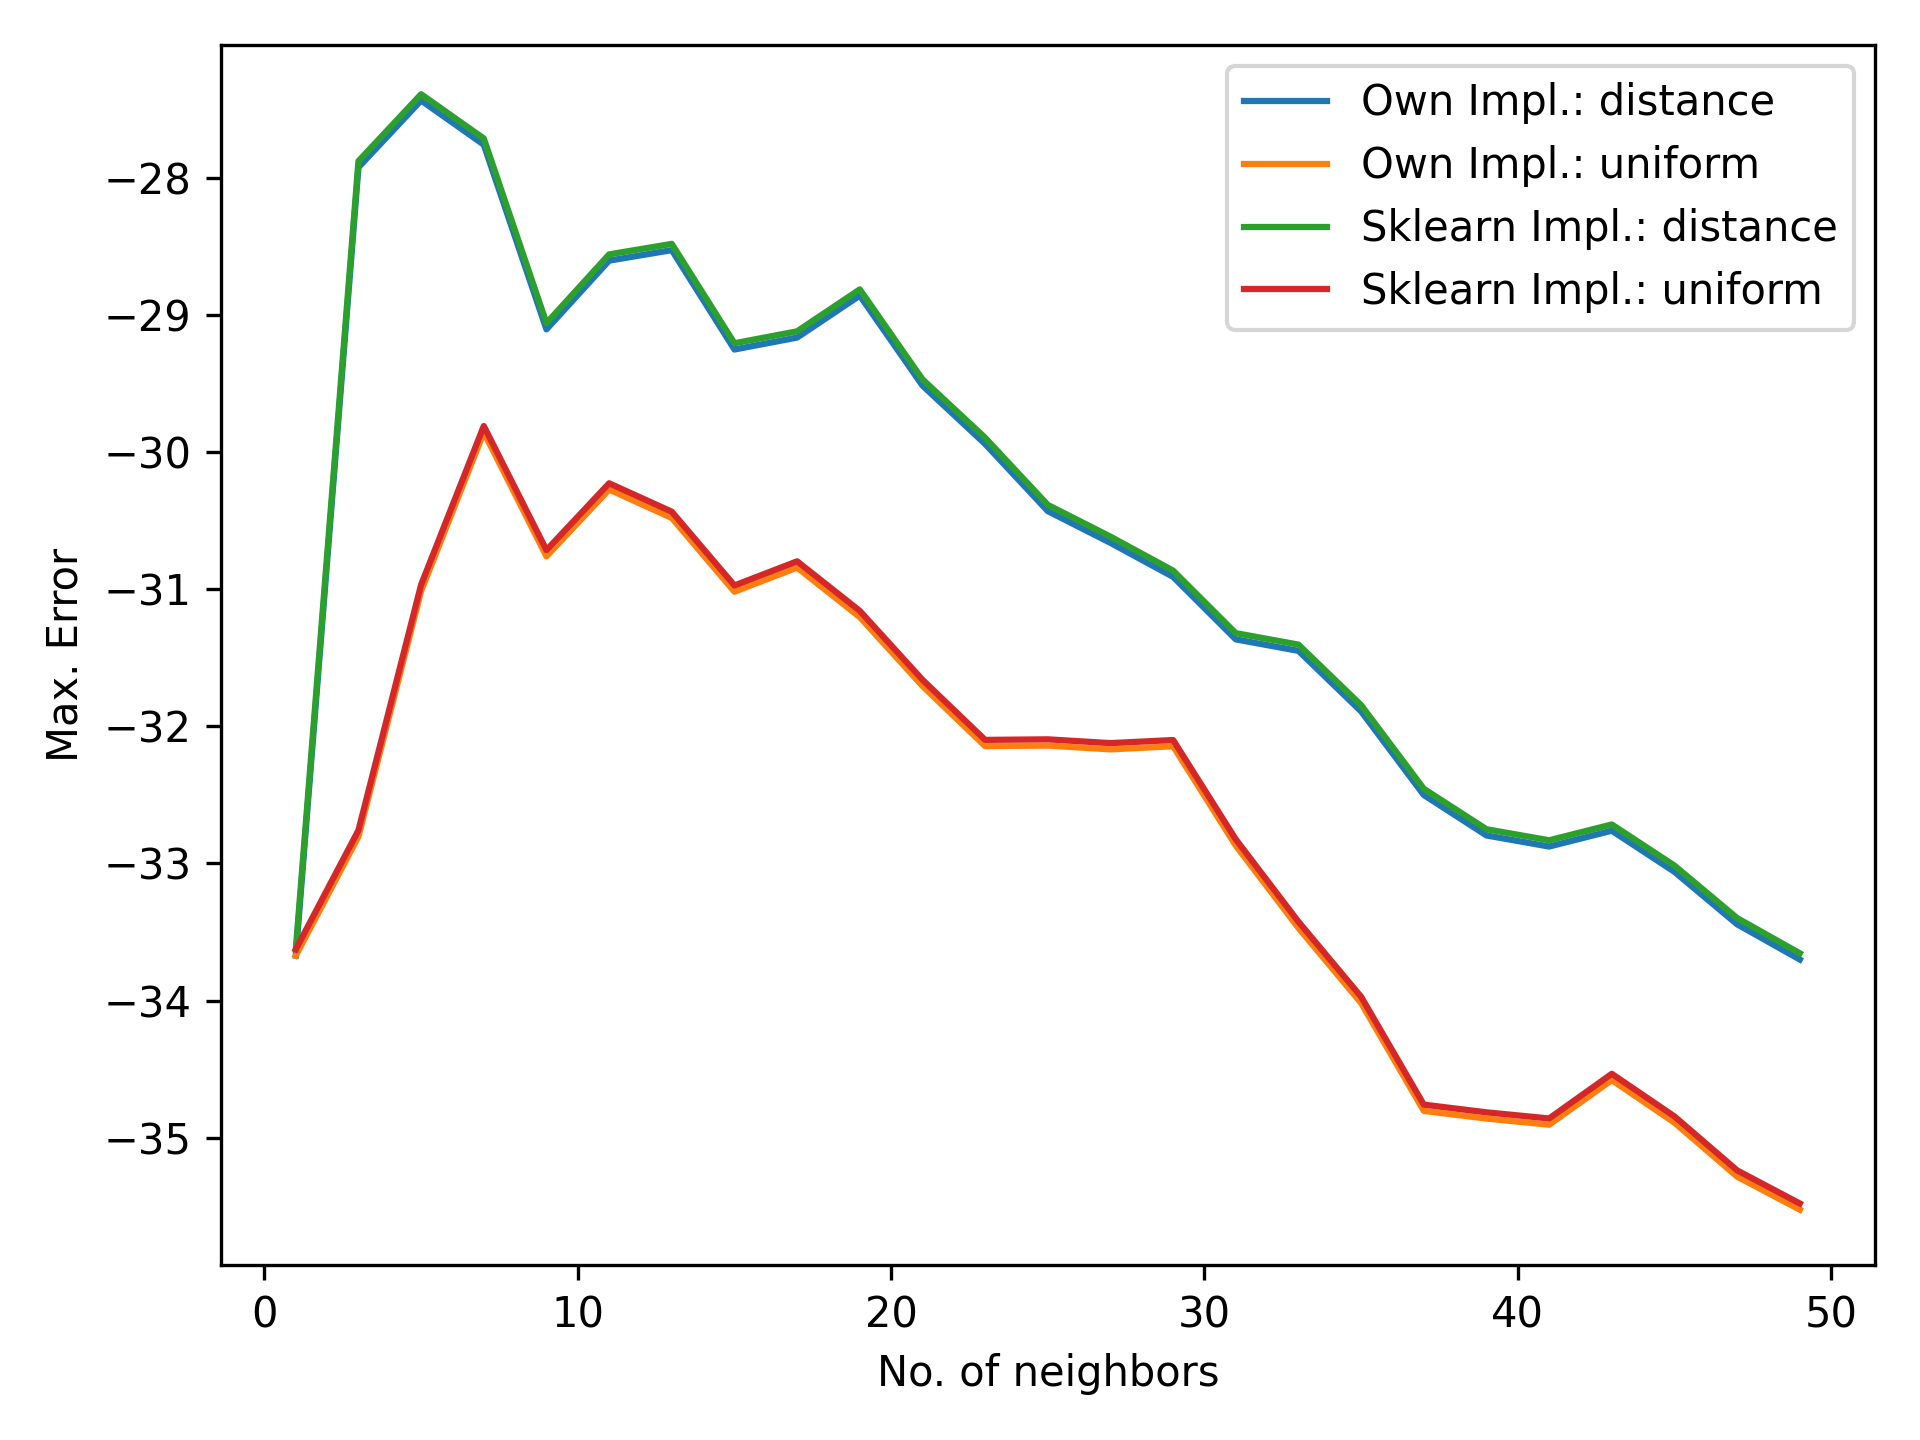
\includegraphics[width=0.8\textwidth]{exercise_2/presentation/figures/concrete_knn_scores_max_error.png}
            \caption{Max. error of $k$-NN on Concrete Data Set}
            \label{fig:kNN_concrete_max-error}
       \end{figure}
    \end{frame}
    
    \begin{frame}{Performance on Life Expectancy Data Set}
        \begin{figure}[h!]
            \centering
            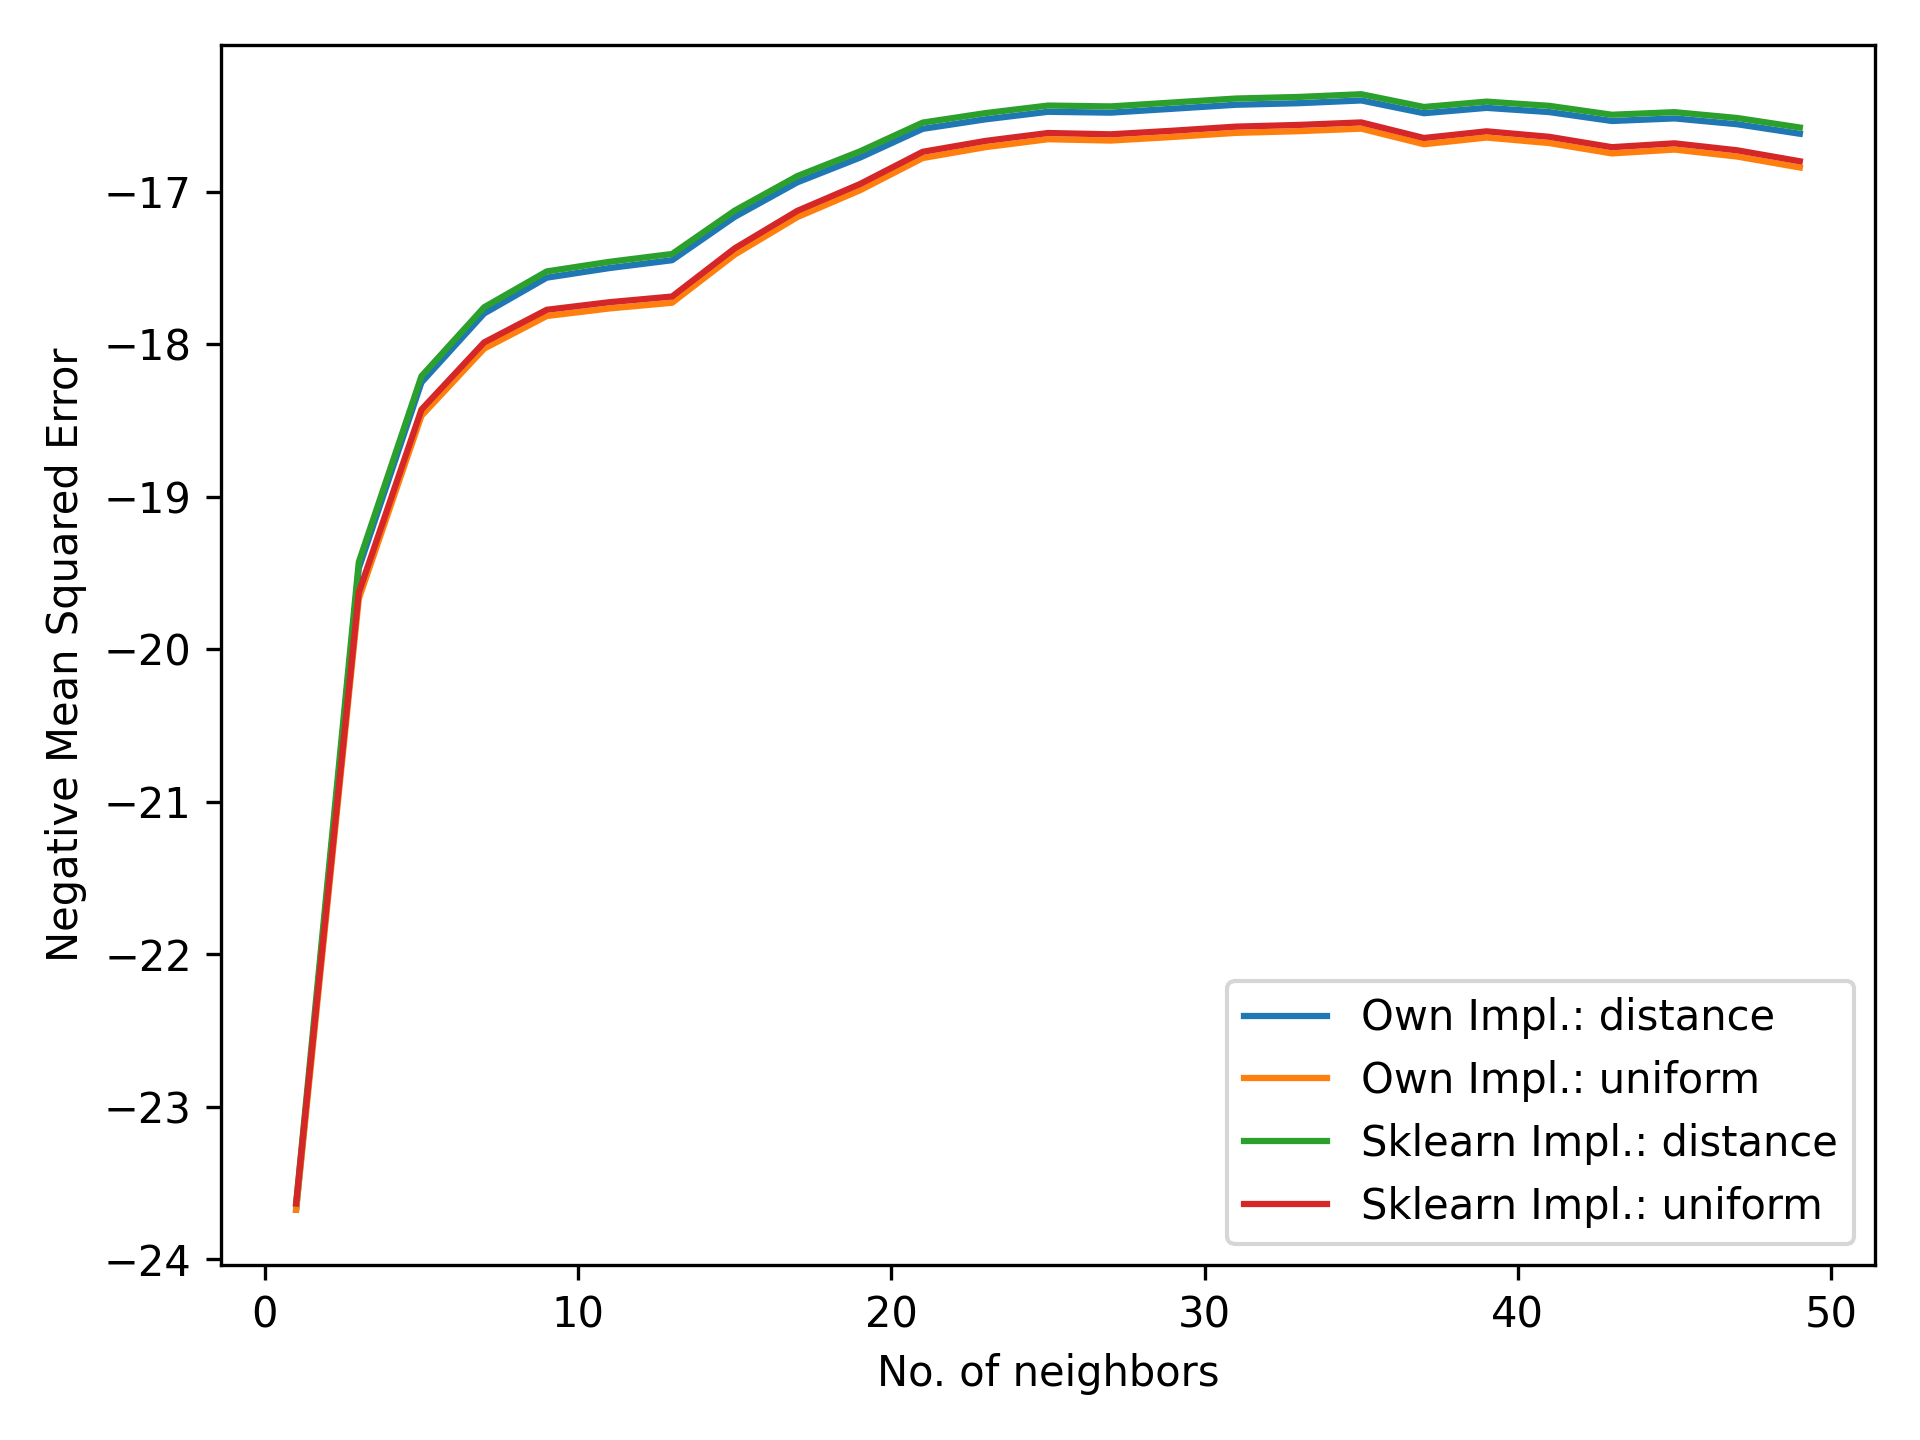
\includegraphics[width=0.8\textwidth]{exercise_2/presentation/figures/le_knn_scores_mean_sq_err.png}
            \caption{MSE of k-NN on Life Expectancy Data Set}
            \label{fig:kNN_LE_MSE}
        \end{figure}    
    \end{frame}
    
    \begin{frame}{Performance on Life Expectancy Data Set}
        \begin{figure}[h!]
            \centering
            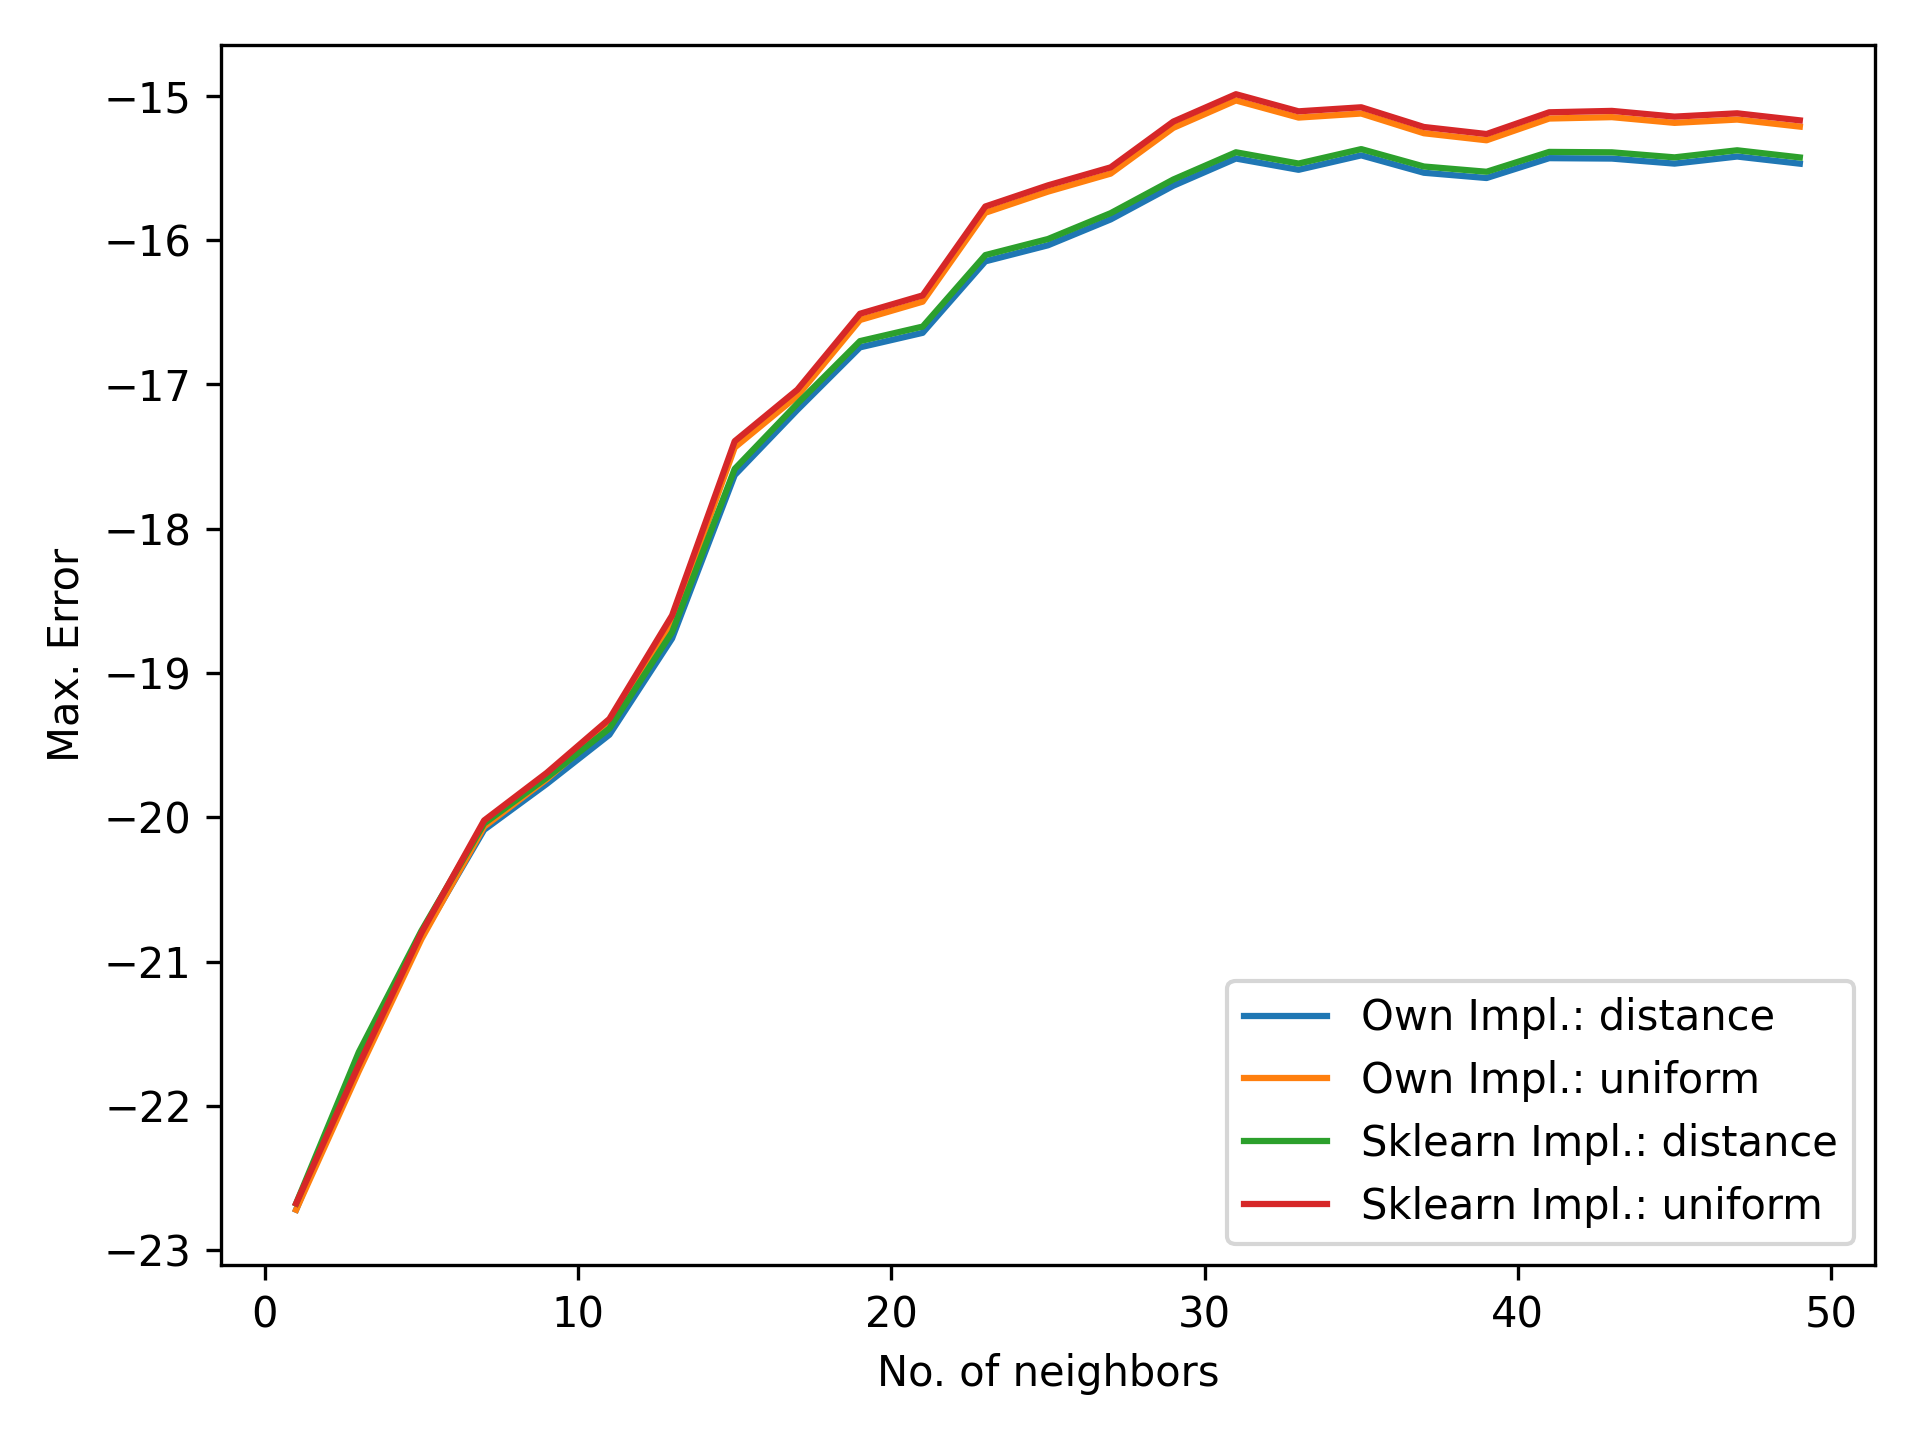
\includegraphics[width=0.8\textwidth]{exercise_2/presentation/figures/le_knn_scores_max_error.png}
            \caption{Max. error of k-NN on Life Expectancy Data Set}
            \label{fig:kNN_LE_max-error}
        \end{figure}    
    \end{frame}
        
    \begin{frame}{Performance on Diamonds Data Set}
        \begin{figure}[h!]
            \centering
            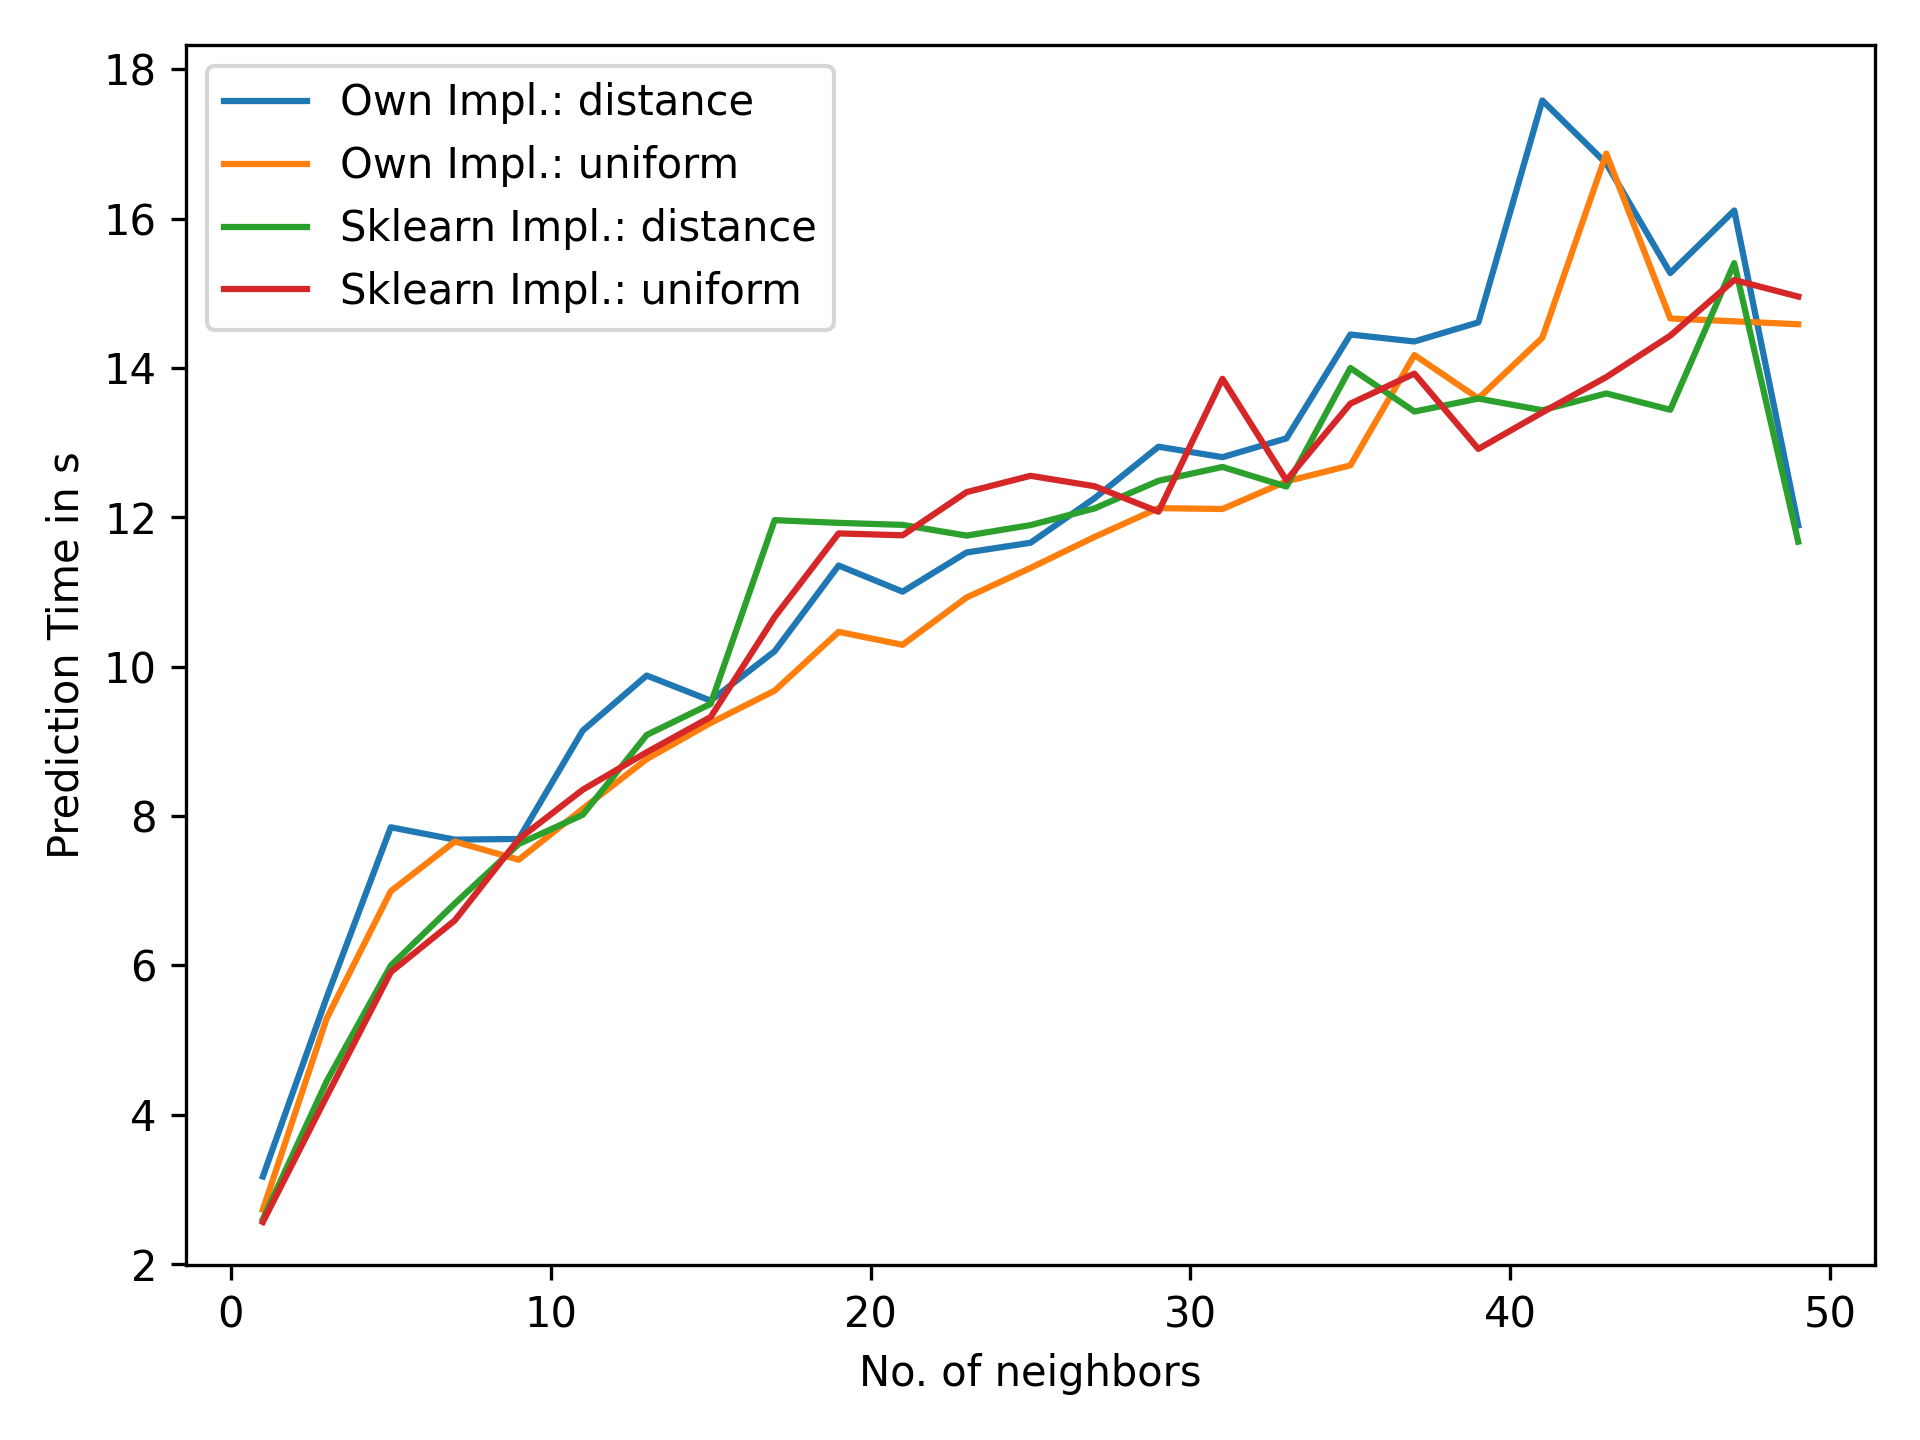
\includegraphics[width=0.8\textwidth]{exercise_2/presentation/figures/diamond_knn_scores_runtime.png}
            \caption{Prediction time of $k$-NN on Diamonds Data Set}
            \label{fig:kNN_Diamond_runtime}
       \end{figure}
    \end{frame}
    
    \begin{frame}{Runtime on Concrete Data Set}
        \begin{figure}[h!]
            \centering
            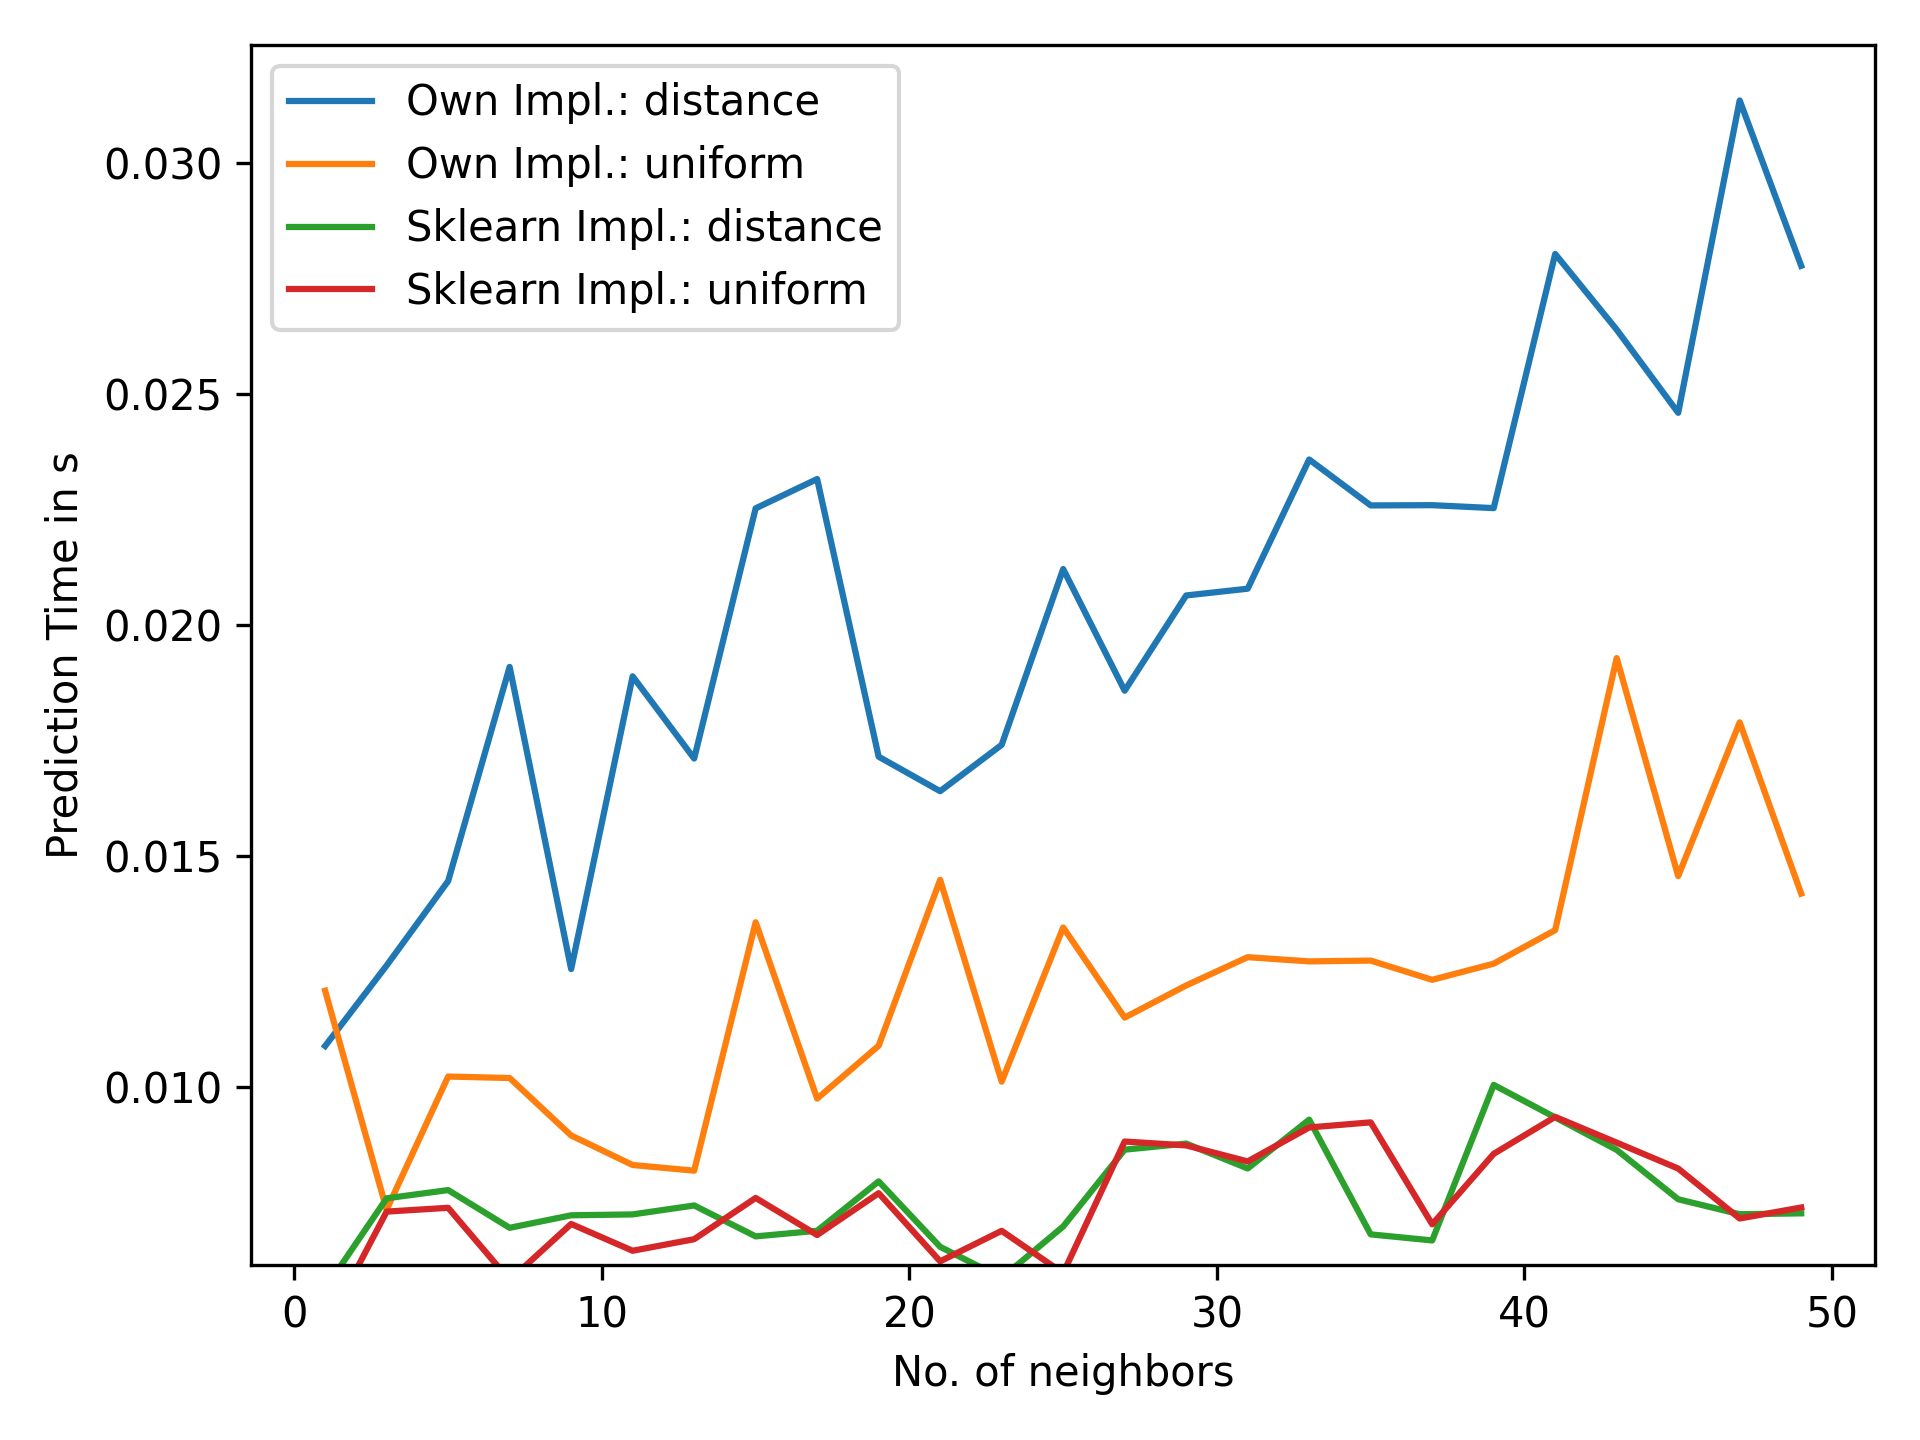
\includegraphics[width=0.8\textwidth]{exercise_2/presentation/figures/concrete_knn_scores_runtime.png}
            \caption{Prediction time of $k$-NN on Concrete Data Set}
            \label{fig:kNN_concrete_runtime}
       \end{figure}
    \end{frame}
    
    \begin{frame}{Runtime on Life Expectancy Data Set}
        \begin{figure}[h!]
            \centering
            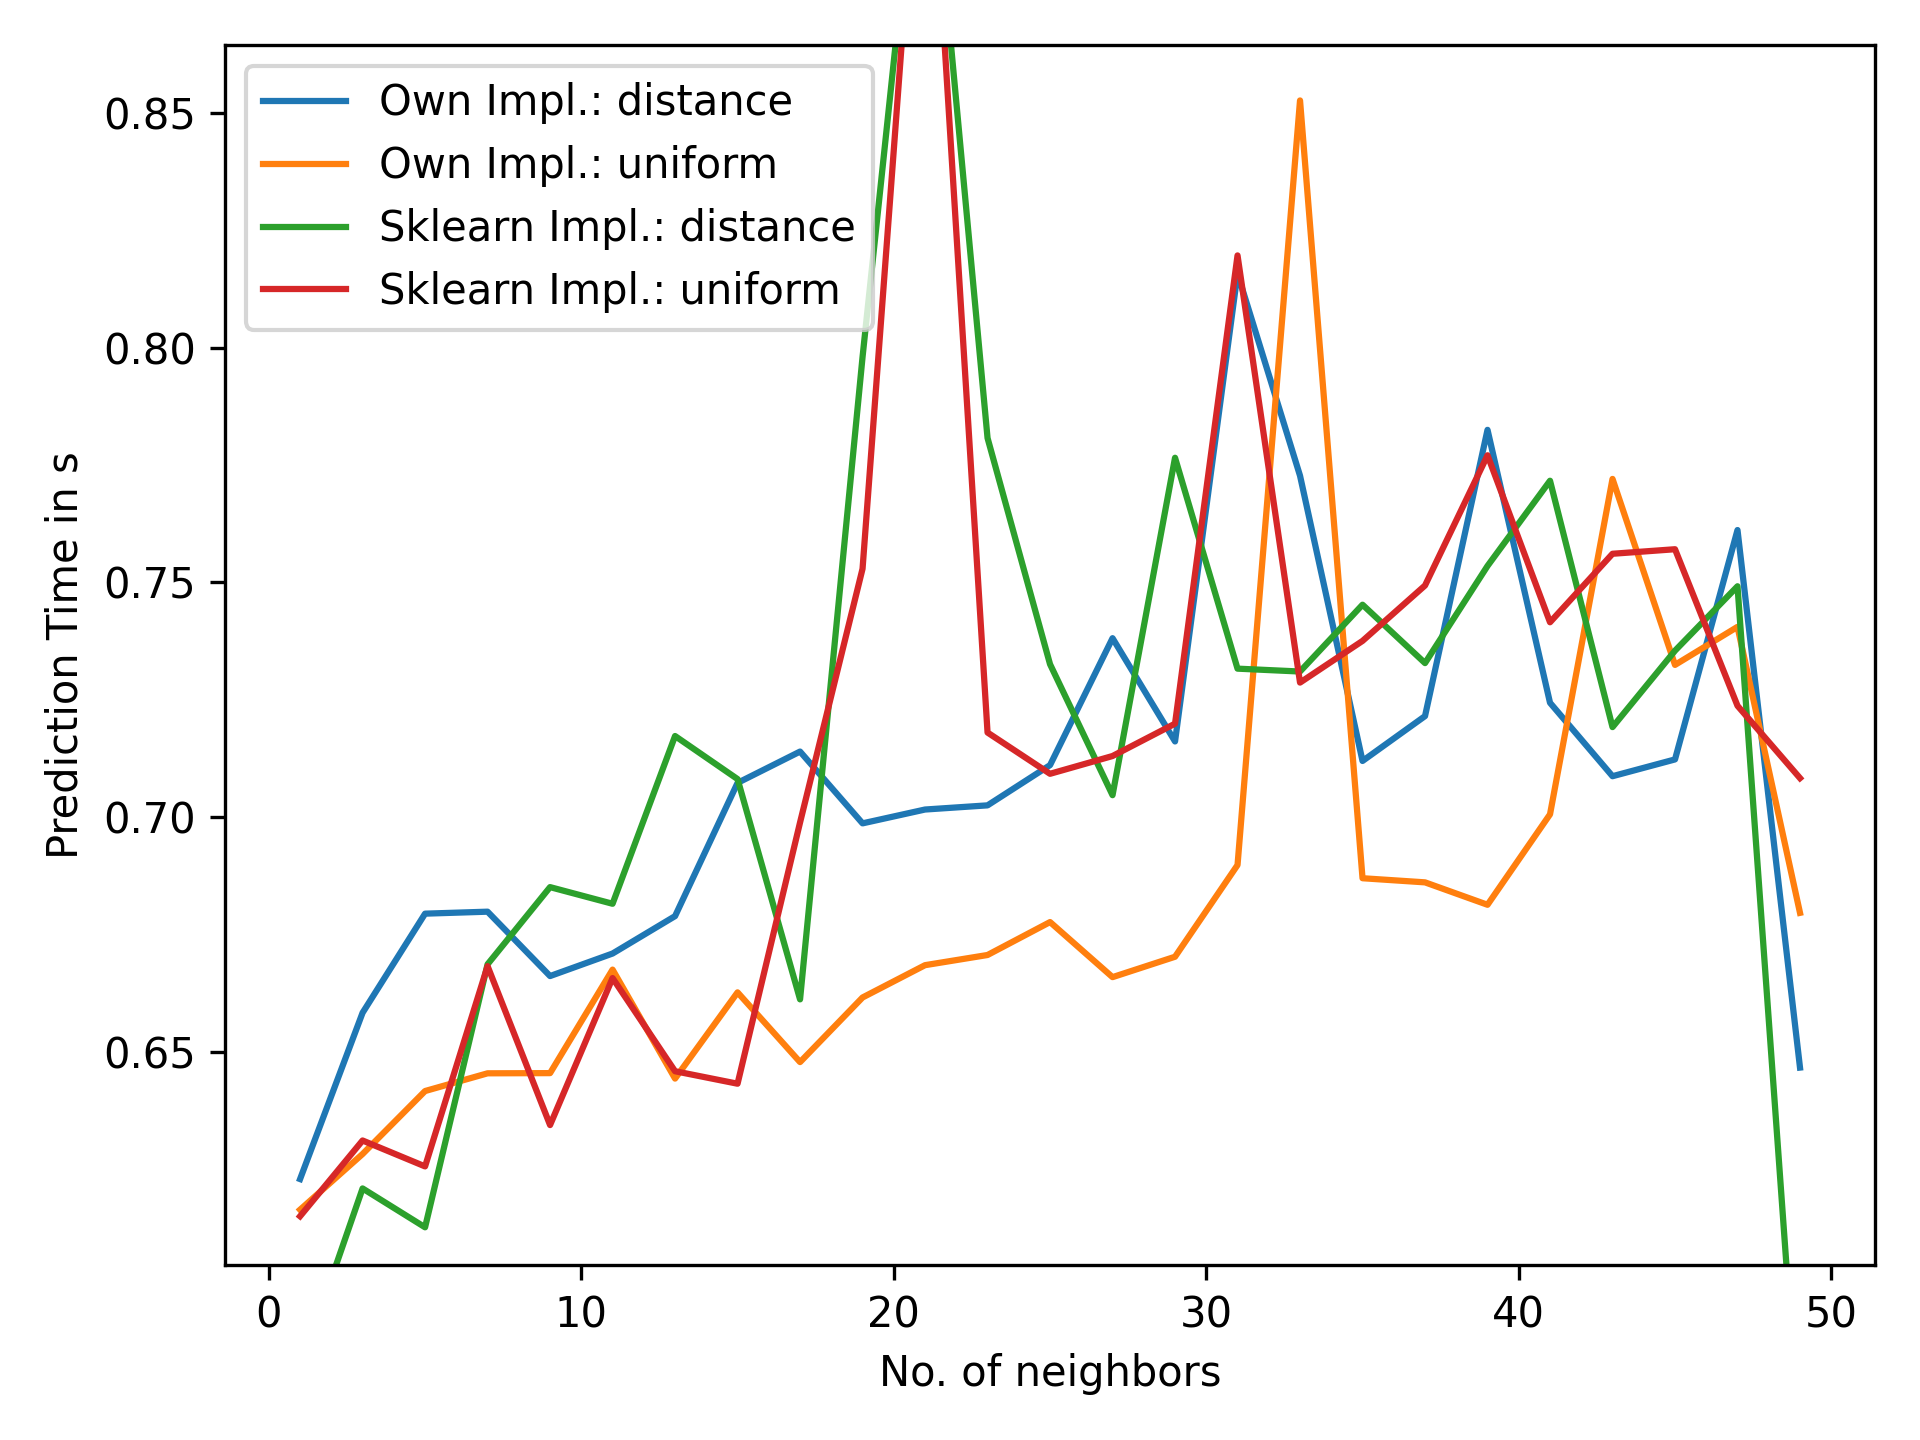
\includegraphics[width=0.8\textwidth]{exercise_2/presentation/figures/le_knn_scores_runtime.png}
            \caption{Prediction time of $k$-NN on Life Expectancy Data Set}
            \label{fig:kNN_LE_runtime}
        \end{figure}    
    \end{frame}

\section[Comparison with other algorithms]{Comparison with other algorithms}
    \begin{frame}[fragile]{Comparison with other algorithms}
        \begin{tabular}{l|c|c|r|c|c|c}
             \multirow{2}{*}{}& \multicolumn{2}{c|}{Diamonds} & \multicolumn{2}{c|}{Concrete} & \multicolumn{2}{c}{Life Expectancy} \\
             & MSE & Max. err. & MSE & Max. err. & MSE & Max. err. \\
                \hline
            $k$-NN & $4.4 \cdot 10^6$ & $9.5 \cdot 10^3$ & 65 & 27 & 16 & 15 \\
                \hline
            GD & $9.9 \cdot 10^6$ & $7.5 \cdot 10^3$ & 109 & 31 & 21 & 20 \\
                \hline
            DT & $3.9\cdot 10^6$ & $8.0 \cdot 10^3$ & 42 & 31 & 14 & 15 \\
                \hline
            RF & $3.5 \cdot 10^6$ & $6.5 \cdot 10^3$ & 25 & 23 & 8 & 12 \\
        \end{tabular}
        
        $k$-NN...implemented $k$-NN \\
        GD...implemented Gradient Descent \\
        DT...Decision tree of sklearn (with default parameters) \\
        RF... Random forest of sklearn (with default parameters)
    \end{frame}
    
\section[Conclusion]{Conclusion}
    \begin{frame}[fragile]{Conclusion Gradient Descent}
        \begin{itemize}
            \item Our implementation was worse than the sklearn implementation regarding the performance metrics, but behaved similar 
            
            \item Additionally, the runtime of our implementation was higher compared to the sklearn version
            
            \item To achieve similar results as in sklearn, a higher number of iterations was needed

            \item Our algorithm worked the best for $\alpha=10^{-2}$ in our tests, across all data sets
            
            \item Standard-Scaling improved the results
        \end{itemize}
    \end{frame}
    
    \begin{frame}[fragile]{Conclusion $k$-NN}
        \begin{itemize}
            \item Our $k$-NN implementation achieved the same results as in sklearn, also with an similar runtime
            
            \item Different optimal $k$ values for different data sets
            
            \item Manhattan distance performed best resp. always really good
            
            \item Using the inverse distance as weights yielded better scores than uniform weights
            
            \item Standard-Scaling improved the results
        \end{itemize}
    \end{frame}
    
\begin{frame}[allowframebreaks]{References}
    \bibliography{demo}
    \bibliographystyle{abbrv}
    
    \bibitem{diamonds}
        Diamonds Data Set: \url{www.openml.org/d/42225}
        
    \bibitem{concrete}
        Concrete Data Set: \url{www.kaggle.com/prokaggler/concrete-data}
    
    \bibitem{life-expectancy}
        Life Expectancy Data Set: \url{www.kaggle.com/kumarajarshi/life-expectancy-who}
\end{frame}
\end{document}
